%%%%%%%%%%%%%%%%%%%%%%%%%%%%%%%%%%%%%%%%%%%%%%%%%%%%%%%%%%%%%%%%%%%%%%%%%%%%%%%%%%%%%%%%%%%%%%%%%%%%%%%%%%%%%%%%%%%%%%%%%%%%%%%%%%%%%%
%%															BAKALÁŘSKÁ PRÁCE														%%
%% 									Zásuvný modul QGIS pro~výpočet erozního smyvu na~orné půdě										%%
%% 															 Radek NOVOTNÝ															%%
%%																																	%%
%% 					(pro formátování využita šablona: http://geo3.fsv.cvut.cz/kurzy/mod/resource/view.php?id=775 ) 					%%
%%%%%%%%%%%%%%%%%%%%%%%%%%%%%%%%%%%%%%%%%%%%%%%%%%%%%%%%%%%%%%%%%%%%%%%%%%%%%%%%%%%%%%%%%%%%%%%%%%%%%%%%%%%%%%%%%%%%%%%%%%%%%%%%%%%%%%
\documentclass[
  12pt,         			% Velikost základního písma je 12 bodů
  a4paper,      			% Formát papíru je A4
  oneside,       			% Oboustranný tisk
  pdftex,				    % překlad bude proveden programem 'pdftex' do PDF
]{report}       			% Dokument třídy 'zpráva'

\newcommand{\Fbox}[1]{\fbox{\strut#1}}

\usepackage[czech, english]{babel}	% použití češtiny a angličtiny
\usepackage[utf8]{inputenc}			% Kódování zdrojových souborů je UTF8

\usepackage[square,sort,comma,numbers]{natbib}

\usepackage{caption}
\usepackage{subcaption}
\captionsetup{font=small}
\usepackage{enumitem} 
\setlist{leftmargin=*} % bez odsazení

\makeatletter
\setlength{\@fptop}{0pt}
\setlength{\@fpbot}{0pt plus 1fil}
\makeatletter

\usepackage[dvips]{graphicx}   
\usepackage{color}
\usepackage{transparent}
\usepackage{wrapfig}
\usepackage{float} 
\usepackage{listings}
\usepackage{placeins} % přidání FloatBarier
\usepackage[justification=centering]{caption} % centrování popisků
\usepackage[font=small,skip=0pt]{caption} %odstranění mezery mezi plovoucím prostředím a popiskem

\usepackage{cmap}           
\usepackage[T1]{fontenc}    

\usepackage{textcomp}
\usepackage[compact]{titlesec}
\usepackage{amsmath}
\addtolength{\jot}{1em} 

\usepackage{chngcntr}
\counterwithout{footnote}{chapter}

\usepackage{acronym}

\usepackage[
    unicode,                
    breaklinks=true,        
    hypertexnames=false,
    colorlinks=true, % true for print version
    citecolor=black,
    filecolor=black,
    linkcolor=black,
    urlcolor=black
]{hyperref}         

\usepackage{url}
\usepackage{fancyhdr}
%\usepackage{algorithmic}
\usepackage{algorithm}
\usepackage{algcompatible}
\renewcommand{\ALG@name}{Pseudokód}% Update algorithm name
\def\ALG@name{Pseudokód}

\usepackage[
  cvutstyle,          
  bachelor           
]{thesiscvut}

\newif\ifweb
\ifx\ifHtml\undefined % Mimo HTML.
    \webfalse
\else % V HTML.
    \webtrue
\fi 

\renewcommand{\figurename}{Obrázek}
\def\figurename{Obrázek}

%%%%%%%%%%%%%%%%%%%%%%%%%%%%%%%%%%%%%%%%%%%%%%%%%%%%%%%%%%%%%%%%%%%%%%%%%%%
%%%%%%%%%%%%%%%%%%%%% Definice informací o dokumentu  %%%%%%%%%%%%%%%%%%%%%
%%%%%%%%%%%%%%%%%%%%%%%%%%%%%%%%%%%%%%%%%%%%%%%%%%%%%%%%%%%%%%%%%%%%%%%%%%%

%% Název práce
\nazev{Zásuvný modul QGIS pro~výpočet~erozního~smyvu~na~orné půdě}
{Soil Loss on Arable Land QGIS Plugin}

%% Jméno a příjmení autora
\autor{Radek}{Novotný}

%% Jméno a příjmení vedoucího práce včetně titulů
\garant{Ing.~Martin~Landa,~Ph.D.}

%% Označení oboru studia
\oborstudia{Geodézie, kartografie a~geoinformatika}{}

%% Označení ústavu
\ustav{Katedra geomatiky}{}

%% Rok obhajoby
\rok{2017}

%Mesic obhajoby
\mesic{červen}

%% Místo obhajoby
\misto{Praha}

%% Abstrakt
\abstrakt 
{Cílem bakalářské práce je návrh softwarového nástroje pro výpočet a prezentaci erozního smyvu na orné půdě, který je podkladem pro agrotechnická a organizační opatření při projektování komplexních pozemkových úprav, případně opatření proti nežádoucím vlivům odtokových poměrů. Výstupem aplikace je rastrový soubor prezentující hodnotu erozního smyvu v tunách na hektar za rok (t/ha.rok) pomocí barevné škály v zájmovém území a souhrnná tabulka obsahující výsledné hodnoty erozně hodnocených ploch. Jako platforma pro vývoj nástroje bude použit programovací jazyk Python, grafický framework PyQt, open source desktopový program QGIS a jeho API (rozhraní pro programovaní aplikací). Nástroj bude implementován ve formě tzv. zásuvného modulu pod licencí GNU GPL.
}
{Abstract in English}

%% Klíčová slova
\klicovaslova
{GIS, QGIS, GRASS, zásuvný~modul, python,  půdní eroze, USLE}
{GIS, QGIS, GRASS, plugin, python, soil erosion, USLE}

%%%%%%%%%%%%%%%%%%%%%%%%%%%%%%%%%%%%%%%%%%%%%%%%%%%%%%%%%%%%%%%%%%%%%%%%

%%%%%%%%%%%%%%%%%%%%%%%%%%%%%%%%%%%%%%%%%%%%%%%%%%%%%%%%%%%%%%%%%%%%%%%%
%% Nastavení polí ve Vlastnostech dokumentu PDF
%%%%%%%%%%%%%%%%%%%%%%%%%%%%%%%%%%%%%%%%%%%%%%%%%%%%%%%%%%%%%%%%%%%%%%%%
\nastavenipdf
%%%%%%%%%%%%%%%%%%%%%%%%%%%%%%%%%%%%%%%%%%%%%%%%%%%%%%%%%%%%%%%%%%%%%%%

%%% Začátek dokumentu
\begin{document}

\catcode`\-=12  % pro vypnuti aktivniho znaku '-' pouzivaneho napr. v \cline 

% aktivace záhlaví
\zahlavi

% předefinování vzhledu záhlaví
\renewcommand{\chaptermark}[1]{%
	\markboth{\MakeUppercase
	{%
	\thechapter.%
	\ #1}}{}}

% Vysázení přebalu práce
%\vytvorobalku

% Vysázení titulní stránky práce
\vytvortitulku

% Vysázení listu zadani
\stranka{}%
	{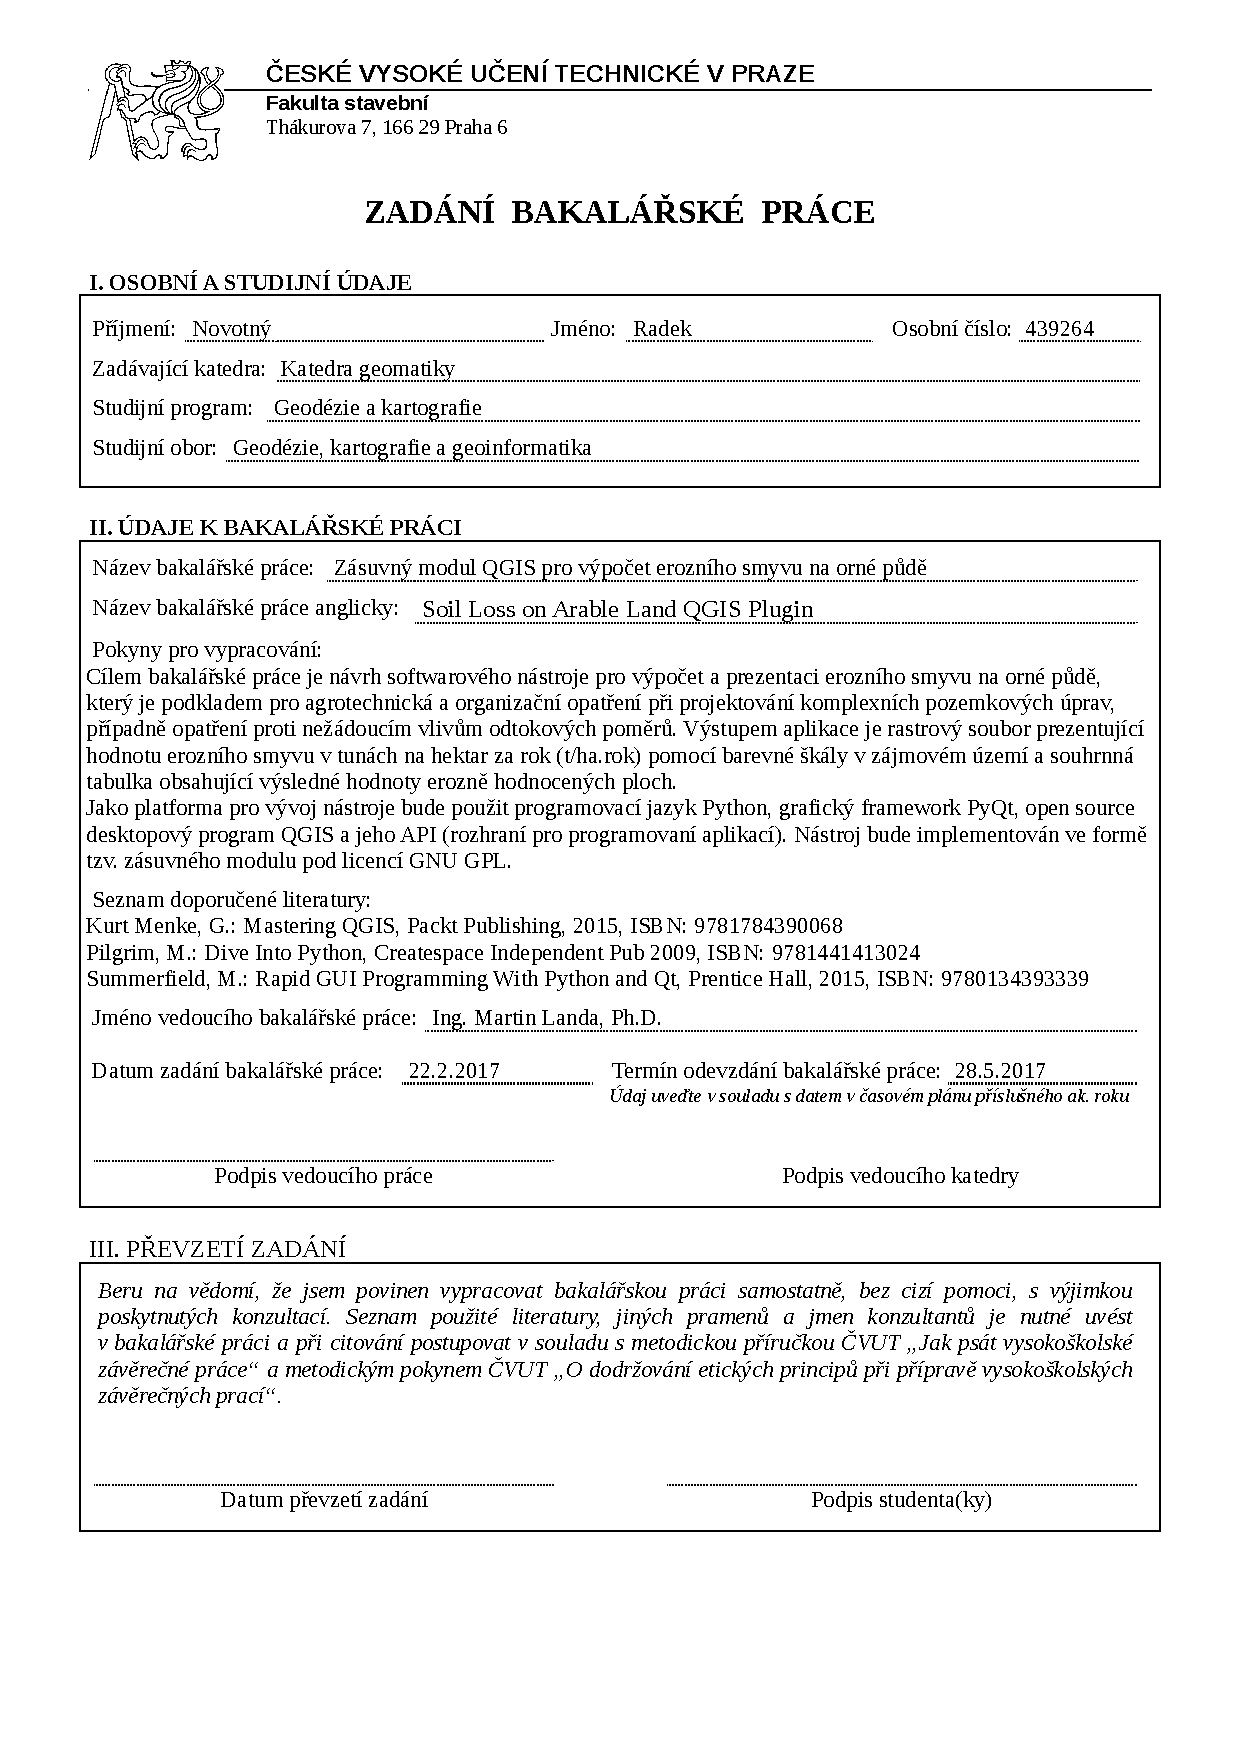
\includegraphics[scale=0.77]{./pictures/zadani.pdf}}%\sffamily\Huge\centering\ }%ZDE VLOŽIT LIST ZADÁNÍ}%
	%{\sffamily\centering Z~důvodu správného číslování stránek}

% Vysázení stránky s abstraktem
\vytvorabstrakt

% Vysázení prohlaseni o samostatnosti
\vytvorprohlaseni

% Vysázení poděkování
\stranka{%nahore
       }{%uprostred
       }{%dole
       \sffamily
	\begin{flushleft}
		\large
		\MakeUppercase{Poděkování}
	\end{flushleft}
	\vspace{1em}
		%\noindent
	\par\hspace{2ex}
	{Podekovani...}
}

% Vysázení obsahu
\obsah

% Vysázení seznamu obrázků
\seznamobrazku

% Vysázení seznamu tabulek
\seznamtabulek

% jednotlivé kapitoly

%!TEX ROOT=radek-novotny-bp-2017.tex
\chapter{Teoretický základ}
\label{2-teorie}
\section{Eroze}
\subsection{Co je eroze?}
\begin{wrapfigure}{l}{0.43\textwidth}
\vspace{-16pt} \centering
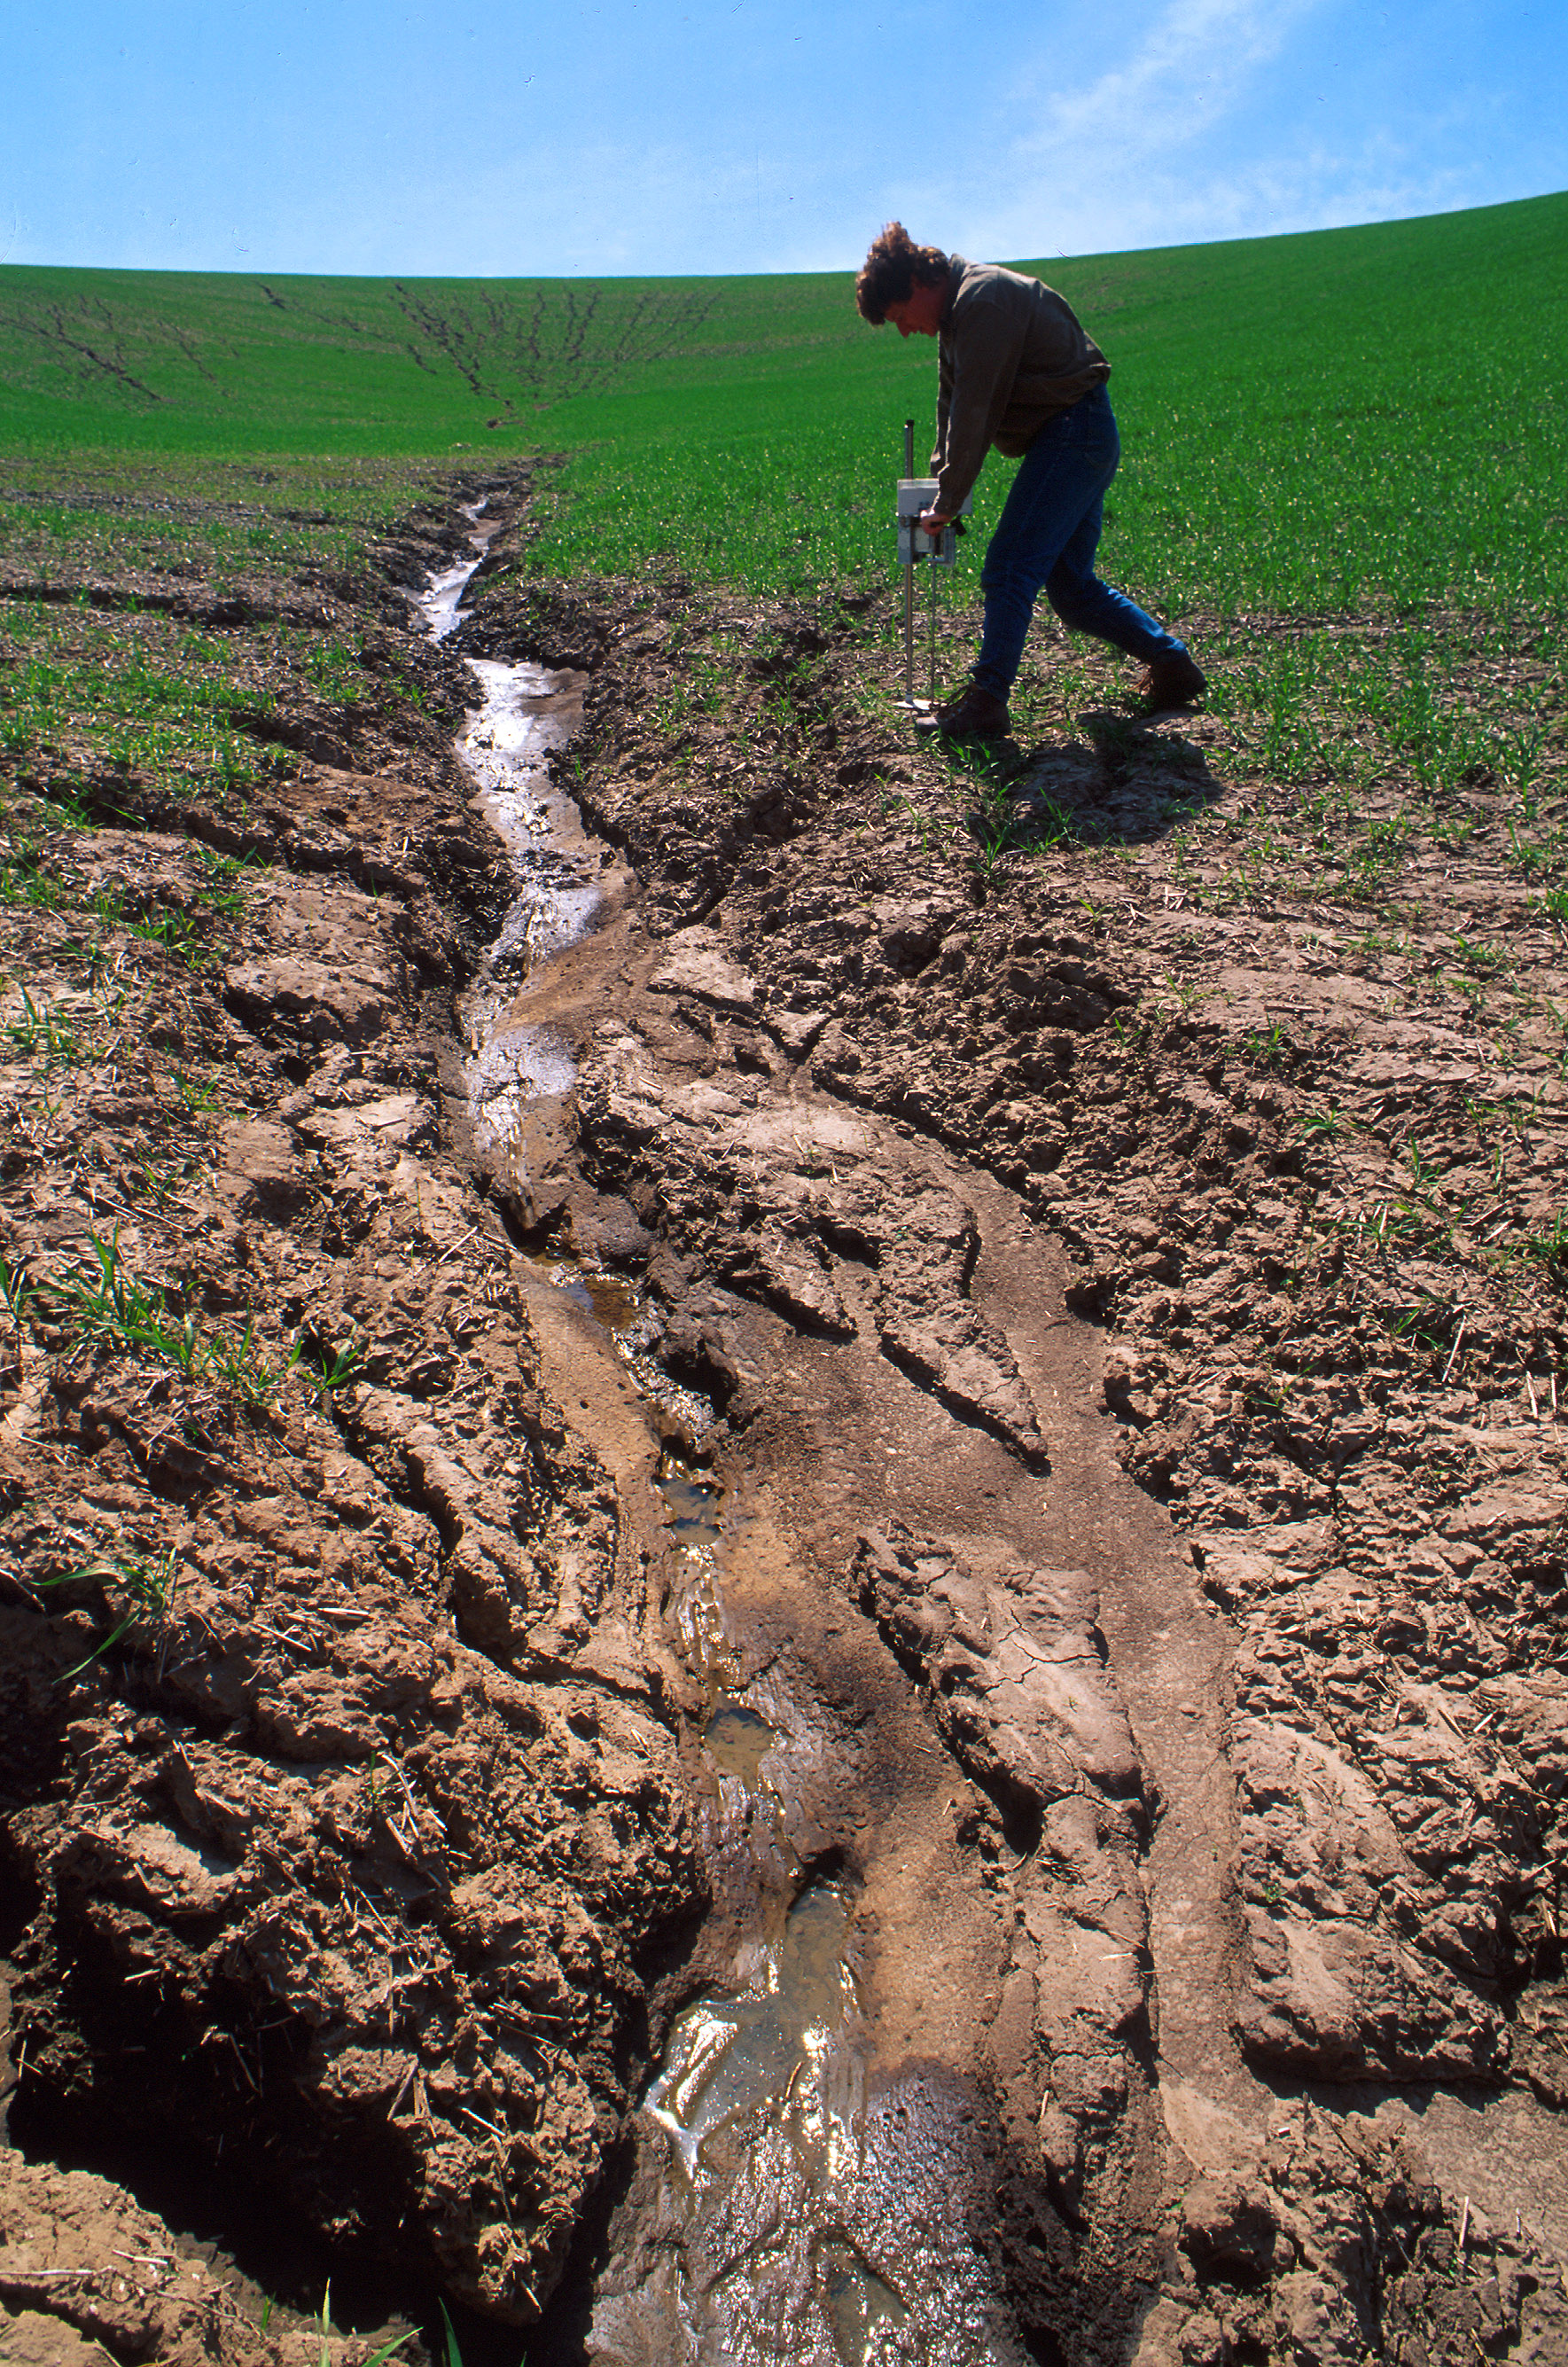
\includegraphics[width=0.43\textwidth]{./pictures/erosion.jpg}
\caption[Ilustrační obrázek eroze]{\label{erosion}Ilustrační obrázek
  eroze zdroj: Wikimedia Commons\cite{wikicommons}}
\vspace{-20pt}
\end{wrapfigure}
Eroze, z latinského „erodere“ – rozhlodávat, je přirozeným přírodním
procesem, během kterého dochází mechanickým působením vnějších faktorů
– vody, větru a sněhu k~rozrušování půdního povrchu, transportu
půdních částic a jejich ukládání na novém místě
(sedimentaci).\cite{Holy1994}

Vliv přirozené neboli geologické eroze není problémem, a naopak je
jedním ze základních procesů tvorby krajiny po milióny let. Dochází
při ní k uvolňování biogenních prvků (např. fosfor, draslík, síra),
jež jsou nezbytné pro život všech organismů a jinak by zůstaly
navázané v horninách. Rychlost geologické eroze je srovnatelná s
rychlostí, kterou je přirozenými procesy vytvářena půda
nová.\cite{Holy1994}

Vlivem antropogenních jevů bohužel nastává tzv. zrychlená půdní eroze,
která má negativní vliv jak na kvalitu půd (zúžení půdního profilu,
snížení obsahu živin, zvýšení štěrkovitosti), jelikož při ní dochází k
odstraňování nejúrodnější složky půdy – ornice, tak na plodiny na ní
pěstované (mechanické poškození, ztráty osiva a~hnojiv). Díky tomu
může na silně erodovaných pozemcích docházet ke ztrátám až 3/4
z~hektarového výnosu. Následná sedimentace půdních částic zanáší vodní
toky, nádrže a při zvýšeném povodňovém průtoku může způsobovat
rozsáhlé škody v intravilánech obcí.\cite{Novotny2014}
\subsection{Rozdělení eroze}
Kromě rozdělení eroze dle intenzity na přirozenou a zrychlenou, je
možné erozi dělit podle činitele, jenž jí způsobuje na erozi vodní,
větrnou a sněhovou.\cite{Holy1994}
\subsubsection{Vodní eroze}
Při vodní (akvatické) erozi dochází k rozrušování zemského povrchu
dopadem vodních kapek, nejsilněji při letních přívalových deštích, kdy
se dopadající voda nestihne vsáknout do půdy a následný povrchový
odtok způsobuje další vymílání a transport půdních částic. Vodní eroze
je v České republice nejčastější a je jí ohroženo více než~50~\%
veškeré orné půdy. Je ovlivněna především sklonem pozemku, délkou
pozemku po spádnici, vegetačním pokryvem a strukturou půdy.

Vodní erozi můžeme dále dělit dle formy odtoku. Jako první probíhá při
dešti plošná eroze (plošný splach), ta je charakteristická
rozrušováním a smyvem půdní hmoty z celého území. Jejím prvním stupněm
je eroze selektivní, při níž jsou povrchovým odtokem odnášeny jemné
půdní částice, na které jsou vázány chemické látky. Tím je způsobena
větší hrubozrnnost a snížení obsahu živin v půdě zasažené
erozí. Naopak půda obohacená smyvem je jemnozrnnější a bohatší na
živiny. Druhý stupeň plošné eroze probíhá při větší kinetické energii
povrchově stékající vody a střídání málo odolných a odolných vrstev,
odtud také název – eroze vrstevná. Projevuje se po celé ploše svahu a
odnáší celé málo odolné vrstvy ornice.

Druhou formou odtoku je výmolová eroze, vznikající postupným
soustřeďováním vody stékající po povrchu a jejím zařezáváním do
půdy. Prvním stádiem je eroze rýžková či brázdová, kdy na povrchu
vznikají úzké rýžky a mělčí širší brázdy, které tvoří na postiženém
území hustou síť. Voda odtékající v soustředěném odtoku má větší
kinetickou energii, čímž transportuje půdu ve větším
rozsahu. Důsledkem stékání rýžek a brázd voda dále získává na síle,
vzniká rýhová eroze. Pokud zesílí mění se v erozi výmolovou či
devastující erozi stržovou, které způsobují hluboké výmoly a
strže.\cite{Novotny2014}
\subsubsection{Větrná eroze}
Druhým nejvýznamnějším typem v ČR je eroze větrná neboli eolická, jež
ohrožuje téměř 10 \% výměry orné půdy. Jedná se území, kde se
vyskytují výsušné větry, pozemky jsou zde sceleny do obrovských
jednotek, na kterých se hospodaří monokulturně a vlivu mechanické síly
větru (abrazi) není bráněno větrolamy, např. oblasti jižní Moravy a
Polabí.

Při větrné erozi dochází k unášení půdních částic různých velikostí,
od velmi jemných zrnek (<0,1 mm), která jsou transportována velmi
snadno ve formě suspenze, často i na velké vzdálenosti a ve větším
množství mohou způsobovat písečné bouře a zákaly atmosféry. Přes
částice střední velikosti (0,1-0,4mm), která představují 50-80\%
celkového objemu přenášeného větrem a způsobují největší škody kolizí
a~rozrušováním vytvořeného půdního agregátu. Po největší zrna (0,5-2
mm), která se pohybují sunutím po povrchu a představují asi 25\%
objemu větrné eroze.\cite{Holy1994}

\subsubsection{Sněhová eroze}
Sněhová eroze transportuje půdní částice obdobně jako eroze vodní,
avšak vyznačuje se určitými specifiky, jedním z nich je zanedbatelný
vliv kinetické energie dopadajících sněhových vloček na rozrušování
povrchu půdy, erozní účinnost sněhu je tedy výhradně při jeho
tání.\cite{Holy1994}

\subsection{Protierozní opatření}
\begin{figure}[H]
    \centering
    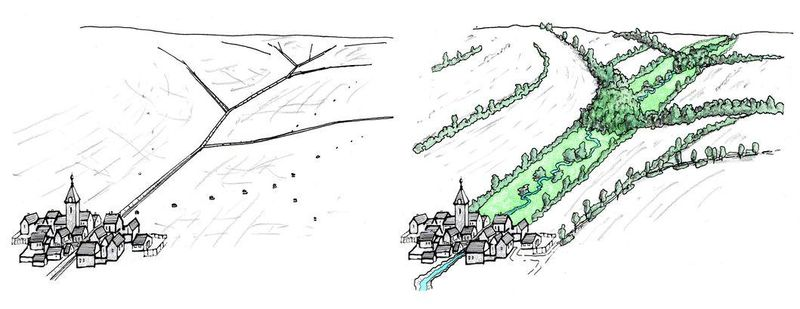
\includegraphics[scale=0.5]{./pictures/protierozni_opatreni.jpg}
      \caption[Ilustrace technického protierozního opatření]{Ilustrace
        technického protierozního opatření, AOPAK ČR\cite{AOPAK} }
      \label{fig:r_faktor_graph}
\end{figure}

Pojem protierozní opatření označuje konkrétní kroky vedoucí k
minimalizaci nega\-tivních dopadů eroze na půdu, vodní toky a nádrže,
intravilán obcí apod. Protierozní opatření dělíme na organizační,
tj. vhodné umístění pěstovaných plodin, pásové střídání plodin nebo
návrhy vegetačních pásů mezi pozemky, agrotechnická (půdoochranné
obdělávání) a technická (příkopy, terasy, protierozní nádrže a
další). Ve většině případů jde o komplex těchto opatření, která se
vzájemně doplňují, aby byly splněny všechny požadavky na ně kladené a
zároveň byly respektovány potřeby zemědělské
výroby.\cite{Holy1994}\cite{janecek2012}

\subsubsection{Organizační protierozní opatření}
Základní organizační protierozní opatření je navržení vhodné velikosti
a tvaru pozem-ku a jeho situování delší stranou po
vrstevnicích. Dodržení tohoto základního pravidla, není vždy
jednoduché, neboť proti sobě působí dva faktory – přírodní, který vede
k vytváření menších pozemků s lepší erozní a ekologickou stabilitou,
a~faktor ekonomický, jenž naopak upřednostňuje tvorbu dostatečně
velkých pozemků pro efektivní využívání zemědělských strojů. Tvar a
velikost pozemku je tedy kompromisem mezi geografickými podmínkami a
požadavky vlastníků (uživatelů) půdy. Obecně se doporučuje navrhování
půdních bloků do 50 ha na rovinných územích a~do~20 ha v územích
členitějších.

Dalším krokem je delimitace (vymezení hranic) druhu pozemků, která
slouží jako funkční a prostorová optimalizace využití pozemků
zemědělského půdního fondu. Ten je rozdělen na ornou půdu, zahrady,
louky, pastviny, vinice, sady a chmelnice. K rozdělení dochází na
základě erozní ohroženosti pozemků, kdy nejohroženější pozemky, které
nemohou být dále využívány jako orná půda, jsou
zatravněny. Umís-těním~trvalého travního porostu by měly být chráněny
také průlehy, ochranné hrázky a břehy vodních toků a nádrží. Je vhodné
umístění liniových pásů travního porostu v drahách výmolové
eroze. Nejúčinnější ochrany proti vodní erozi je dosaženo zalesněním
území, optimálně lesem smíšeným.

Důležitým faktorem je tedy přítomnost vegetačního pokryvu, jehož
význam je nejvyšší v období letních přívalových dešťů. Vegetace chrání
půdu před přímým dopadem dešťových kapek, podporuje vsak vody do půdy
a její kořenový systém pomáhá zvyšovat soudržnost půdy vůči stékající
vodě. Těchto znalostí se využívá při výběru dalších organizačních
opatření, kterými mohou být např. včasný výsev plodin, posunutí
podmítky do období s nižším výskytem přívalových dešťů (tj. na září),
zařazení bezorebně setých meziplodin a v neposlední řadě rozmístění
plodin dle ohroženosti pozemku, kdy pozemky rovinné nebo mírně
sklonité je vhodné využít pro pěstování plodin nedostatečně chránících
půdu před erozí (širokořádkové plodiny) a pro pozemky více ohrožené
volit plodiny s lepším protierozním charakterem nebo pásové střídání
plodin, kdy se střídají pásy plodin chránících půdu (např.~travní
porost, vojtěška, jetel) s plodinami s nižší protierozní účinností
(okopaniny, kukuřice).\cite{janecek2012}

\subsubsection{Agrotechnická protierozní opatření}
Jelikož nejvíce ohrožena erozí je půda bez vegetačního pokryvu, snaží
se agrotechnická protierozní opatření zkrátit období, kdy je půda
obnažena na minimum. Nej\-rizikovějšími obdobími jsou zejména období
tání sněhu a letních přívalových dešťů. Úspěšným prostředkem je cílené
využívání biomasy z meziplodin a posklizňových zbytků, přičemž je
třeba dbát na neomezování možnosti infiltrace vody do půdy.

Mezi nejúčinnější způsoby patří technologie ochranného zpracování
půdy, kdy je místo orby využíváno kypření půdy bez obracení
zpracovávané vrstvy půdy. Ovšem i při orbě lze snížit vliv vodní eroze
dodržením pravidla o orání ve směru vrstevnic, kdy brázdy mohou omezit
povrchový odtok vody. Dále existuje množství dalších technologií, jež
jsou specifické pro pěstované plodiny, jejich přehled je možné najít v
metodice Ochrana zemědělské půdy před
erozí\cite{janecek2012}(str. 60-70).\cite{Holy1994}

\subsubsection{Technická protierozní opatření}
Technické prvky jsou základem protierozní ochrany, a to především tam,
kde smyv z~pozemků má důsledky pro intravilán obce. Jedná se o
převážně liniové prvky, které jsou optimálně rozmisťovány tak, aby
došlo k přerušení délky svahu a rozčlenění pozemků. Dále mají vliv na
agrotechnické opatření, kdy usměrňují směr obdělávání pozemků a způsob
hospodaření jejich uživatelů. Vhodná je i jejich kombinace s
organizačními opatřeními, kdy po rozdělení svahu liniovými opatřeními
jsou do nově vymezených pásů umístěny plodiny s různou protierozním
povahou. V neposlední řadě je jejich funkce i ekologického a krajině
estetického charakteru. Technická protierozní opatření jsou navrhována
během pozemkových úprav a patří mezi ně průlehy, příkopy, hrázky,
meze, ochranné nádrže, stabilizování drah soustředného odtoku a
terasování. Způsoby navrhování zmiňovaných opatření lze dohledat
v~meto-dice Ochrana zemědělské půdy před
erozí\cite{janecek2012}(str. 70-90). Dále lze čerpat z
\cite{Kadlec2014}\cite{Novotny2014}.
\newpage
\section{Historie}
\subsection{Počátky výzkumu eroze}
Výzkumem eroze se začali zabývat vědci v USA začátkem 20. století,
jednou z~významných osobností při prvních krocích výzkumu byl Hugh
Bennett, který začal pozorovat zvýšenou erozi na zemědělské půdě a
její vliv na výnos. Bennett na tento rostoucí problém veřejně
upozorňoval, do většího povědomí se však ochrana zemědělské půdy
dostala až na přelomu 20. a 30. let v souvislosti s mohutnými
prachovými bouřemi (tzv. Dust Bowl, Dirty Thirties).\cite{usda_ars}
\begin{figure}[H]
    \centering 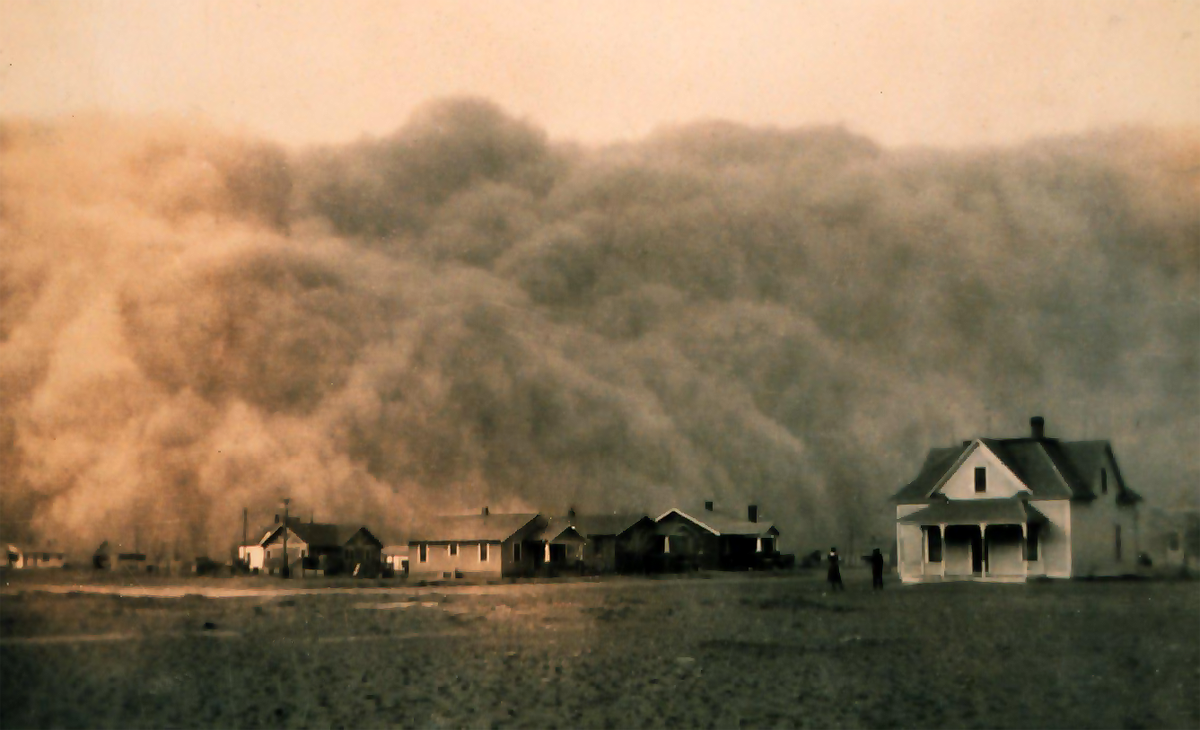
\includegraphics[scale=0.7]{./pictures/Dust_bowl.png}
      \caption[Foto bouře v oblasti Dust Bowl z roku 1935]{Foto bouře
        v oblasti Dust Bowl z roku 1935, zdroj: Wikimedia
        Commons\cite{wikicommons}}
      \label{fig:dust_bowl}
\end{figure}

\paragraph{Dust Bowl,} slovní spojení, jež bylo původně použito pro oblast vzniku prachových
bouří - Velkých planin a následně se stalo synonymem i pro období
30. let (proto také druhý název Dirty Thirties), kdy se bouře
objevovaly. Příčinou byla rychlá změna suchých prérií s nízkým
srážkovým úhrnem (místy pod 250 mm/rok) na zemědělskou půdu. Tuto
změnu umožnilo rozšíření zemědělských strojů, zejména traktorů, díky
kterým mohla být na rozsáhlém území využita hluboká orba, kterou byla
zničena původní vegetace chránící půdní povrch. Místo původních travin
byla na většině území vysazena pšenice, přičemž nebylo dodržováno ani
střídavé hospodaření.

Ve spojení s nulovou ochranou půdy došlo tímto způsobem zemědělství v
obdobích sucha k proměně půdy v prach, který byl unášen větrem a
vytvářel mohutná prachová oblaka devastující krajinu. Erozí zasáhla
okolo 100 milionů akrů půdy (v~roce 1934 bylo bouří zasaženo dokonce
východní pobřeží USA včetně New Yorku), zanechala bez domova téměř 500
tisíc lidí a způsobila stěhování až 3,5 milionu lidí ze zasažené
oblasti, čímž se jednalo o největší migrační vlnu v historii
USA. Touto katastrofou byla dále prohloubena Velká hospodářská krize.

První reakcí bylo v roce 1929 zřízení deseti výzkumných stanic, ve
kterých byla na tzv. jednotkových pozemcích (délka 22,13 m, sklon
9$\%$, trvalý úhor, obdělávání ve směru sklonu) pozorována eroze a
měřen smyv. Z měření byla regresní analýzou odvozeny faktory
ovlivňující erozi a účinnost ochranných opatření. Další krok učinil v
roce 1932 nově zvolený americký prezident Franklin Roosevelt, který v
rámci opatření proti trvající hospodářské krizi zřídil úřad zabývající
se půdní erozí (SES – Soil Erosion Service), v čele kterého stanul
H. Bennett. Tento úřad začal učit farmáře šetrnějším metodám
hospodaření, budovat velké množství protierozních opatření, při čemž
zaměstnával dělníky zasažené ekonomickou depresí, a samozřejmě
pokračoval ve výzkumu eroze.\cite{Bonnifield1979}\cite{Egan2006}

\subsection{Vývoj USLE}
\begin{figure}[H]
    \centering 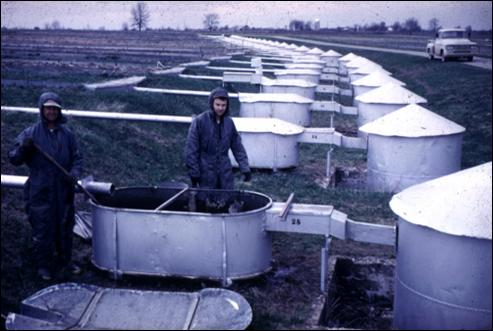
\includegraphics[scale=0.85]{./pictures/unit_plots.jpg}
      \caption[Foto jednotkových pozemků v Missouri v 50. letech]{Foto
        jednotkových pozemků v Missouri v 50. letech, zdroj: USDA
        ARS\cite{usda_ars}}
      \label{fig:unit_plots}
\end{figure}
Díky studiím z výzkumných stanic, které postupně vznikaly, bylo
shromážděno velké množství informací, které byly dále využity pro
výpočty erozního smyvu. Vývoj matematických rovnic pro odhad množství
půdní eroze a vliv ochranných opatření začal v druhé polovině
30. let. První empirický model(\ref{zing1940}) pro odhad průměrné
roční ztráty půdy způsobené vodní erozí publikoval v roce 1940
A. W. Zingg. Jeho rovnice zahrnovala vliv sklonu pozemku a jeho
délku. Konstanty byly určovány pro kukuřičný pás (Corn Belt), hlavní
zemědělskou oblast USA.\cite{ZINGG1940}
\begin{align}
   \label{zing1940} G=L^{0,6}\cdot S^{1,4}\cdot C
\end{align}
\hspace*{2cm}$G \cdots$ průměrná roční ztráta půdy\\
\hspace*{2cm}$L \cdots$ délka svahu \\
\hspace*{2cm}$S \cdots$ sklon svahu \\
\hspace*{2cm}$C \cdots$ koeficient zahrnující ostatní faktory\\

Tento model v roce 1941 rozšířil D. D. Smith, který do rovnice
(\ref{smith1941}) zahrnul vliv technických protierozních
opatření. Smith jako první využil její výsledky využil k určení
maximální délky svahu na specifickém území a stanovení metod
ochrany.\cite{Smith1941}
\begin{align}
   \label{smith1941} G=L^{\frac{3}{5}}\cdot S^{\frac{7}{5}}\cdot P\cdot C
\end{align}
\hspace*{2cm}$G \cdots$ průměrná roční ztráta půdy\\
\hspace*{2cm}$L \cdots$ délka svahu \\
\hspace*{2cm}$S \cdots$ sklon svahu \\
\hspace*{2cm}$P \cdots$ faktor protierozních opatření \\
\hspace*{2cm}$C \cdots$ koeficient zahrnující ostatní faktory \\

Tato rovnice byla G. M. Browning použita pro sestavení empirického
modelu pro stát Iowa (\ref{browning}), kde jsou poprvé zahrnuty
geologické faktory půdy a agrotechnických opatření.\cite{browning1947}
\begin{align}
   \label{browning} G=10\cdot\left( K^{\prime}\cdot O^{\prime}\cdot  L^{\prime}\cdot S^{\prime}\cdot C^{\prime}\cdot P^{\prime} \right)
\end{align}
\hspace*{2cm}$G \cdots$ průměrná roční ztráta půdy\\
\hspace*{2cm}$K^{\prime} \cdots$ faktor erodovatelnosti půdy \\
\hspace*{2cm}$O^{\prime} \cdots$ faktor geologického podkladu \\
\hspace*{2cm}$L^{\prime} \cdots$ délka svahu \\
\hspace*{2cm}$S^{\prime} \cdots$ sklon svahu \\
\hspace*{2cm}$C^{\prime} \cdots$ faktor vegetačního pokryvu \\
\hspace*{2cm}$P^{\prime} \cdots$ faktor protierozních opatření \\

V roce 1947 Musgrave publikoval první erozní
model(\ref{musgrave1947}), který zahrnoval vliv přívalového deště. V
této rovnici byly také překlasifikovány hodnoty faktorů pro kukuřičný
pás.\cite{MUSGRAVE1947}

\begin{align}
   \label{musgrave1947} G=K\cdot C\cdot L^{0,35}\cdot S^{1,35}\cdot R^{1,75}
\end{align}
\hspace*{2cm}$G \cdots$ průměrná roční ztráta půdy\\
\hspace*{2cm}$K \cdots$ geologický faktor eroze půdy \\
\hspace*{2cm}$C \cdots$ faktor vegetačního pokryvu \\
\hspace*{2cm}$L \cdots$ délka svahu \\
\hspace*{2cm}$S \cdots$ sklon svahu \\
\hspace*{2cm}$R \cdots$ úhrn deště s periodicitou 0,5 za 30 minut \\
\begin{figure}[H]
    \centering
    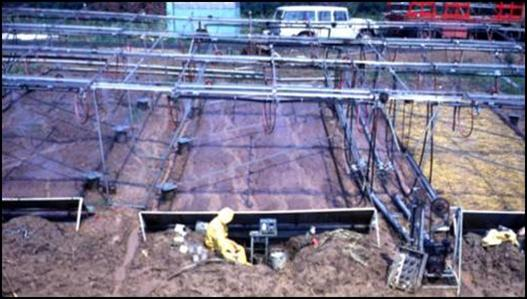
\includegraphics[scale=0.85]{./pictures/unit_plots2.jpg}
      \caption[Foto jednotkových pozemků v Indianě (1968)]{Foto
        jednotkových pozemků v Indianě (1968), zdroj: USDA
        ARS\cite{usda_ars}}
      \label{fig:unit_plots}
\end{figure}
V roce 1954 na Purdue University, která měla v té době vedoucí
postavení v~oblasti výpočetních technologií, vzniklo pod vedením
W. H. Wischmeier centrum pro shromažďování dat o půdní erozi (Soil
Loss Data Center). Přístup k nejmodernějším technologiím dovolil
zrychlit analyzování velkého množství dat (v letech 1940-1965 přes
10~000 zmonitorovaných smyvů ročně), jež byly shromažďovány od
30. let. Výsledkem byla v roce 1965 první kompletní publikace
vytvořená týmem pod vedením Wischmeier a Smith, která byla ještě
zpřesněna dalším výzkumem a upravena do současné formy(\ref{usle1978})
publikované v roce 1978.\cite{usle1978}

\begin{align}
   \label{usle1978} G=R\cdot K\cdot L\cdot S\cdot C\cdot P
\end{align}
\hspace*{2cm}$G \cdots$ průměrná roční ztráta půdy $\left( t\cdot
ha^{-1}\cdot rok^{-1} \right)$\\
\hspace*{2cm}$R \cdots$ faktor erozní účinnosti deště \\
\hspace*{2cm}$K \cdots$ geologický faktor eroze půdy \\
\hspace*{2cm}$L \cdots$ faktor délky svahu \\
\hspace*{2cm}$S \cdots$ faktor sklonu svahu \\
\hspace*{2cm}$C \cdots$ faktor vegetačního pokryvu \\
\hspace*{2cm}$P \cdots$ faktor protierozních opatření \\

\subsection{Modifikace USLE}
\subsubsection{RUSLE}
V roce 1997 byla publikována Revidovaná univerzální rovnice ztráty
půdy (Revised Universal Soil Loss Equation), ta byla odvozena na
základě revize, prověření a aktualizace USLE. Došlo
zde k významné změně způsobu určení erozních faktorů (např. zpřesnění
časového průběhu hodnot R faktoru v patnáctidenním intervalu,
zpřesnění časového průběhu K faktoru v důsledku zhutňování povrchu a
rozpadu půdních agregátů srážkami či obhospodařováním, nové vztahy pro
LS faktor). Výhodou využití RUSLE je tedy přesnější určení
%%% ML: to zavani zastaralosti zdroje, ktery jste pouzil
%%% RN: zrejme zbytecne, odstraneno
erozního modelu. Nevýhodou je nutnost většího množství vstupních
dat.\cite{rusle1997}
\subsubsection{MUSLE}
Druhou významnou úpravou je Modifikovaná univerzální rovnice ztráty
půdy (Modified Universal Soil Loss Equation), která zahrnuje
transportní činitele během erozního procesu a stanovuje množství
splavenin z přívalového deště v povodí do velikosti
15~km$^{2}$.\cite{musle1945}

%%% ML: tato kapitola se tyka ciste CR, je to tak? Pokud ano, tak by
%%% to mel zohlednit jeji nazev
%%% RN: CR se tyka pouze prvni polovina prvniho odstavce, zbytek by
%%% mel platit obecne, nazvem a strukturu kapitoly jeste promyslim
\newpage
\subsection{Současný stav}
USLE je v současnosti používána pro výpočet dlouhodobé eroze ve
%%% ML: opravdu jedinou?
%%% RN: pro vypocet dlouhodobe eroze ano, dale existuji simulacni
%%% modely pro vypocet eroze kratkodobe, zrejme tuto kapitolu ale
%%% jeste uppravim
většině států světa a je jedinou doporučenou metodou v ČR (Metodika
VÚMOP\cite{janecek2012}), existují k ní rozsáhlá katalogová data. Jsou
vytvořeny postupy pro její výpočet v softwarech GIS a je přímo
implementována pro automatické zpracování programy jako jsou USLE2D či
modulem Eroze pro Atlas DMT. Ovšem i přes úpravy a postupné zlepšení
schopnosti odhadu dlouhodobé ztráty půdy je USLE i další zmíněné
metody empirické, tedy založené na využití koeficientů získaných při
pozorování v terénu (na jednotkových pozemcích). Jejich přesnost je
tedy závislá na přesnosti klasifikace jednotlivých faktorů pro
specifickou situaci.

V posledních letech je snaha omezit zavedený empirický základ při
posuzování erozních procesů a nahradit ho kvalitnějšími simulačními
metodami. Cílem této změny je hodnotit důsledky eroze nejen vůči
zemědělské půdě, ale i vůči jiným ekologickým celkům (např. vodní
toky, nádrže) a také řešení eroze na kratším časovém horizontu.  K
vývoji a zdokonalování simulačních modelů přispívá rozvoj výpočetní
techniky, geografických informačních systémů a rozšiřování znalostí v
dané oblasti.\cite{janecek2012}
\begin{figure}[H]
    \centering
    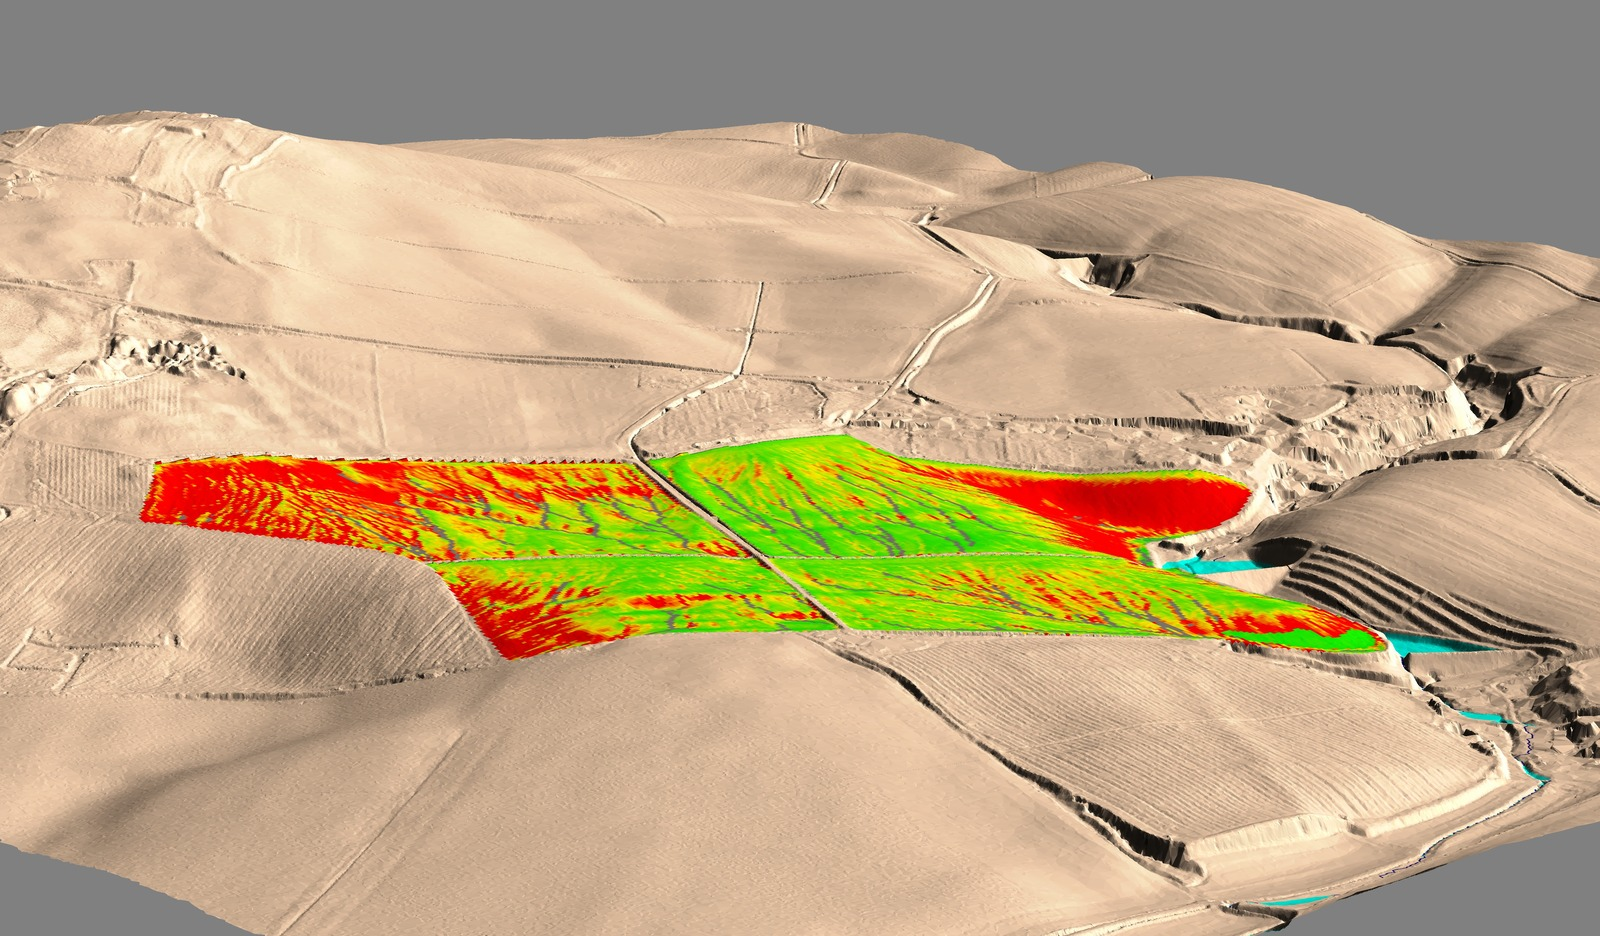
\includegraphics[scale=0.25]{./pictures/atlas_eroze.jpg}
      \caption[Ukázka z výpočtu v GIS aplikaci Eroze pro Atlas
        DMT]{Ukázka z výpočtu v GIS aplikaci Eroze pro Atlas DMT,
        zdroj: Atlas DMT\cite{atlas_e}}
      \label{fig:atlas_eroze}
\end{figure}

\section{Univerzální rovnice ztráty půdy}
\subsection{Faktor erozní účinnosti přívalového deště (R)}
I přesto, že významnější rýhová eroze je pozorována zejména po
neobvykle silných přívalových deštích, během výzkumu byla prokázána
nutnost při odhadu průměrné roční ztráty půdy uvažovat i deště se
střední intenzitou. Pro \zk{usle} byl použit vztah odvozený
Wischmeierem\cite{Wischmeier1959}, který nejlépe aproximoval hodnoty
působení faktoru deště získané z jednotkových pozemků při stálosti
ostatních faktorů. V tomto vztahu nebyl zahrnut smyv při zavlažování
či působení sněhové eroze (tání, obleva), která může být významná v
horských oblastech v jarním období a pro její určení je nutné využít
speciální vztah.

Pro určení srážkového erozního faktoru jsou využity deště oddělené od
sebe alespoň 6~hodin, přičemž nejsou uvažovány ty s úhrnem nižším než
12,5~mm~(0,5 palce) nebo 6,25~mm~(0,25 palce) za~15 minut, jelikož
jejich vliv je zanedbatelný.

Dle definice je hodnota R (v anglické literatuře též označováno jako
parametr EI) dána součinem kinetické energie deště s jeho maximální
30minutovou intenzitou~(\ref{r_factor_1}). Jelikož se ukázalo, že
samotná energie nedostatečně popisuje destruktivní vliv dopadajících
kapek na půdní povrch.\cite{usle1978}
\begin{align}
   \label{r_factor_1} R=E\cdot  \frac{i_{30}}{100}
\end{align}
\hspace*{2cm}$R \cdots$ faktor erozní účinnosti deště $\left( MJ\cdot
ha^{-1}\cdot cm \cdot h^{-1} \right)$\\
\hspace*{2cm}$E \cdots$ celková kinetická energie deště $\left( J\cdot
m^{-2} \right)$\\
\hspace*{2cm}$i_{30} \cdots$ maximální 30minutová intenzita deště
$\left( cm\cdot h^{-1} \right)$\\

Celková kinetická energie deště je sumou ze všech úseků
deště~(\ref{r_factor_2}), kdy jednotlivá kinetická energie závisí na
intenzitě a úhrnu~(\ref{r_factor_3}).\cite{usle1978}
\begin{align}
   \label{r_factor_2} E=\sum_{i=1}^n E_{i}
\end{align}
\begin{align}
   \label{r_factor_3} E_{i}=\left( 206+87 \log i_{si} \right) \cdot H_{si}
\end{align}
\hspace*{2cm}$E_{i} \cdots$ kinetická energie i-tého úseku deště
$\left( J\cdot m^{-2} \right)$\\
\hspace*{2cm}$i_{si} \cdots$ intenzita i-tého úseku deště $\left(
cm\cdot h^{-1} \right)$\\
\hspace*{2cm}$H_{si} \cdots$ úhrn v i-tém úseku deště $\left( cm
\right)$\\

Na základě vypočtených hodnot byla pro USA vytvořena mapa zobrazující
pomocí izolinií průměrné hodnoty R faktoru. \cite{usle1978} V ČR je
dle platné metodiky doporučeno využívat průměrnou
hodnotu.\cite{janecek2012}

Ta byla původně stanovena na 20 $MJ\cdot ha^{-1}\cdot cm \cdot
h^{-1}$. Vycházela z měření na třech stanicích a úhrn dešťů, jež
byly použity pro výpočet, byly sníženy o 12,5 mm. Po použití dat z více
stanic a provedení lepšího metodického rozboru erozní účinnosti deště
bylo určeno, že R faktor se na většině zemědělsky využívaném území ČR
pohybuje mezi hodnotami 30 až 45 $MJ\cdot ha^{-1}\cdot cm \cdot
h^{-1}$., pročež je doporučeno volit tento faktor jako konstantní
hodnotu 40 $MJ\cdot ha^{-1}\cdot cm \cdot h^{-1}$.\cite{janecek2012}

Regionalizovaná mapa(obr. \ref{fig:r_faktor}) s nejnovějšími hodnotami
R faktoru lze najít na serveru SOWAC-GIS.\cite{sowac}

\begin{figure}[H]
    \centering 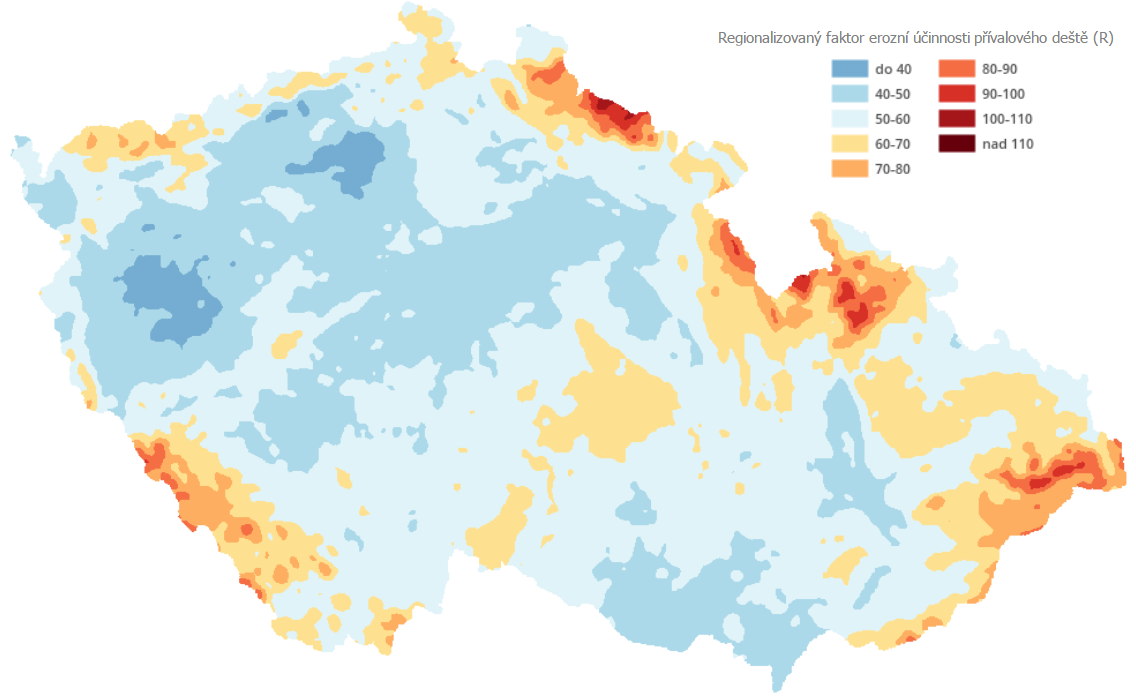
\includegraphics[scale=0.5]{./pictures/r_factor.png}
      \caption{Regionalizované rozdělení faktoru R}
      \label{fig:r_faktor}
\end{figure}

\subsection{Faktor struktury půdy (K)}
Faktor erodovatelnosti půdy udává náchylnost půdy, jako samotné
matérie, k erozi. Měření probíhalo na jednotkových pozemcích
ponechaných ladem, přičemž ostatní faktory (kromě faktoru R, kterým
byla celková eroze vydělena) byly rovny jedné. Jedná se o
komplikovanou proměnou závislou na struktuře, textuře a dalších
fyzic\-kých i chemických vlastnostech zeminy.\cite{usle1978}

První možností, jak faktor erodovatelnosti můžeme určit, je přibližně
podle hlavní půdní jednotky (HPJ) bonitačního půdního systému
(tab. \ref{hpj_k}) nebo Taxonomického klasifikačního systému půd
ČR\cite{Nemecek2001}, jež je rovněž tabelován\cite{janecek2012}. Jedná
se o obdobné řešení jako v původním modelu pro USA, kdy byly vybrány
hlavní půdní typy, pro které byl K faktor určen.\cite{usle1978}

\begin{table}[hbt]
\begin{center}
\catcode`\-=12
    \noindent\begin{tabular}{|*{8}{c|}} \hline \bf HPJ & \bf K & \bf
    HPJ & \bf K & \bf HPJ & \bf K& \bf K & \bf HPJ\\ \hline \bf 1
    &0,41 &\bf 19&0,33 &\bf 36&0,26 &\bf 54&0,40 \\ \hline \bf 2 &0,46
    &\bf 20&0,28 &\bf 37&0,16 &\bf 55&0,25 \\ \hline \bf 3 &0,35 &\bf
    21&0,15 &\bf 38&0,31 &\bf 56&0,40 \\ \hline \bf 4 &0,16 &\bf
    22&0,24 &\bf 40&0,24 &\bf 57&0,45 \\ \hline \bf 5 &0,28 &\bf
    23&0,25 &\bf 41&0,33 &\bf 58&0,42 \\ \hline \bf 6 &0,32 &\bf
    24&0,38 &\bf 42&0,56 &\bf 59&0,35 \\ \hline \bf 7 &0,26 &\bf
    25&0,45 &\bf 43&0,58 &\bf 60&0,31 \\ \hline \bf 8 &0,49 &\bf
    26&0,41 &\bf 44&0,56 &\bf 61&0,32 \\ \hline \bf 9 &0,60 &\bf
    27&0,34 &\bf 45&0,54 &\bf 62&0,35 \\ \hline \bf 10&0,53 &\bf
    28&0,29 &\bf 46&0,47 &\bf 63&0,31 \\ \hline \bf 11&0,52 &\bf
    29&0,32 &\bf 47&0,43 &\bf 64&0,40 \\ \hline \bf 12&0,50 &\bf
    30&0,23 &\bf 48&0,41 &\bf 67&0,44 \\ \hline \bf 13&0,54 &\bf
    31&0,16 &\bf 49&0,35 &\bf 68&0,49 \\ \hline \bf 14&0,59 &\bf
    32&0,19 &\bf 50&0,33 &\bf 70&0,41 \\ \hline \bf 15&0,51 &\bf
    33&0,31 &\bf 51&0,26 &\bf 71&0,47 \\ \hline \bf 16&0,51 &\bf
    34&0,26 &\bf 52&0,37 &\bf 72&0,48 \\ \hline \bf 17&0,40 &\bf
    35&0,36 &\bf 53&0,38 &\bf 73&0,48 \\ \hline \bf 18&0,24 & & & & &
    & \\ \hline
    \end{tabular}\\
    \vspace{10px} Vynechané HPJ nemají K faktor určen kvůli nedostatku
    dat.
  \caption[Hodnoty K faktoru pro jednotlivé HPJ]{Hodnoty K faktoru pro
    jednotlivé HPJ dle metodiky \cite{janecek2012}.}
  \label{hpj_k}
\end{center}
\end{table}
\FloatBarrier Druhou a přesnější metodou, je použití definovaného
vztahu, který je podrobně rozebrán Janečkem\cite{janecek2012} na
str. 13, či použití z něho odvozeného
nomogramu(obr.\ref{fig:k_faktor}). Ovšem pro toto věrnější určení K
faktoru je nezbytné mít k dispozici výsledky rozborů půdy z daného
území.\cite{janecek2012}

\begin{figure}[H]
    \centering
    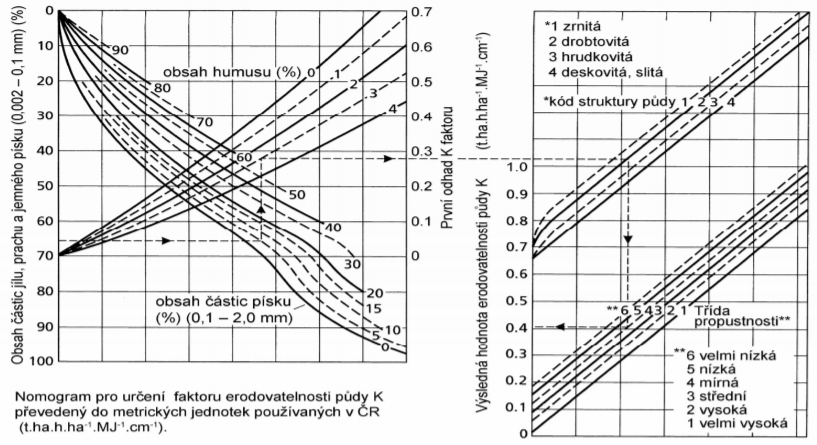
\includegraphics[scale=0.85]{./pictures/k_faktor_nomogram.png}
      \caption[Nomogram pro stanovení K faktoru]{Nomogram pro
        stanovení K faktoru (zdroj: Janeček\cite{janecek2012})}
      \label{fig:k_faktor}
\end{figure}
\subsection{Topografický faktor (LS)}
I přestože faktory sklonu a délky svahu byly zkoumány odděleně a oba
jsou reprezentovány vlastní rovnicí pro výpočet eroze, jsou často
uváděny jako jeden tzv. topografický faktor.\cite{usle1978}

Původní a dodnes využívanou metodou pro jeho určení je výpočet v
tzv. reprezentativních odtokových drahách, které jsou voleny od místa
vzniku povrchového odtoku, tedy rozvodnice či hrany pozemku, pokud je
tento pozemek erozně izolován, po místo, kde se plošná eroze mění v
soustředný odtok. Dále už není možné pro výpočet eroze použít metodu
USLE, jelikož slouží pouze pro výpočet plošné eroze. Také není
doporučeno, aby délka rozvodnice přesáhla 400 m, jelikož výsledky USLE
pro větší délky nejsou ověřeny.\cite{janecek2012}

\subsubsection{Faktor délky svahu - L} 
Při použití reprezentativních odtokových drah se faktor L určí pomocí
vztahu (\ref{l_faktor}), který byl definován v RUSLE\cite{rusle1997} a
jehož výsledkem je poměr ztráty půdy na jednotku plochy svahu ke
ztrátě na jednotkovém pozemku (délka 22,13 m, sklon
9\%).\cite{janecek2012}
\begin{align}
   \label{l_faktor} L=\left( \frac{l}{22,13} \right)^m
\end{align}
\hspace*{2cm}$l \cdots$ horizontální projekce nepřerušené délky svahu
$\left( m \right)$ \\
\hspace*{2cm}$m \cdots$ exponent náchylnosti svahu ke vzniku rýžkové
eroze dle sklonu svahu, tabelovaný v RUSLE\cite{rusle1997} \\
\subsubsection{Faktor sklonu svahu - S} 
Obdobně je tomu u vztahu pro faktor sklonu svahu, jež se liší pro
sklony nižší než 9\% (\ref{s_faktor1}) a slony větší
(\ref{s_faktor2}). Tyto vztahy byly taktéž uvedeny v
RUSLE\cite{rusle1997}.
\begin{align}
   \label{s_faktor1} S=10,8\cdot\sin\Theta + 0,03
\end{align}
\vspace{-40pt}
\begin{align}
   \label{s_faktor2} S=16,8\cdot\sin\Theta - 0,50
\end{align}
\hspace*{2cm}$\Theta \cdots$ úhel sklonu svahu $\left( rad \right)$

\subsubsection{Výpočet faktoru LS s využitím GIS} 
Druhou metodou je výpočet LS faktoru s pomocí GIS, kdy je výpočet
proveden pro mikropovodí v každém pixelu. Pro výpočet LS faktoru
existuje celá řada definovaných vztahů, jejichž porovnáním se zabýval
Krása\cite{Krasa2010}. Pro české podmínky se používá s dostatečnou
přesností rovnice(\ref{ls_faktor}) odvozená
Mitášovou\cite{Mitasova1998}.\cite{Dostal2014}
\begin{align}
   \label{ls_faktor} LS_{x,y}=\left( m+1 \right)\cdot\left(\frac{A_{x,y}}{22,13}\right)^m \cdot \left(\frac{\sin b_{x,y}}{0,09}\right)^n
\end{align}
\hspace*{2cm}$LS_{x,y} \cdots$ LS faktor pixelu o souřadnicích x, y
\\ \hspace*{2cm}$A \cdots$ jednotková zdrojová plocha na vstupu do
buňky $\left( m^2\cdot bm^{-1} \right)$ \\
\hspace*{2cm}$b \cdots$ sklon buňky $\left( rad \right)$ \\
\hspace*{2cm}$m \cdots$ kalibrační parametr, obvykle 0,6\\
\hspace*{2cm}$n \cdots$ kalibrační parametr, obvykle 1,3\\

Při výpočtu jsou klíčovými faktory určení rastru zdrojových ploch,
přičemž by neměl být použit model s jednosměrným odtokem, a zohlednění
přerušení povrchového odtoku.\cite{Krasa2010}
\newpage
\subsection{Faktor ochranného vliv vegetace (C)}
Vegetační faktor se uplatňuje především přímou ochranou půdy před
dopadajícími dešťovými kapkami, dále zpomaluje povrchový odtok,
zpevňuje půdu kořenovým systémem a nepřímo se vlivem vegetace mění i
vlastnosti půdy.

Účinnost ochranného vlivu vegetace se projevuje zejména v období
zvýšeného výskytu přívalových dešťů
(obr. \ref{fig:r_faktor_graph}). Nejdokonaleji půdu chrání les,
vysokou protierozní účinnost mají též traviny a
jeteloviny. Nedostatečně půdu chrání širokořádkové plodiny jako je
kukuřice nebo okopaniny a téměř vůbec není půda chráněna na vinicích a
chmelnicích.
\begin{figure}[H]
    \centering
    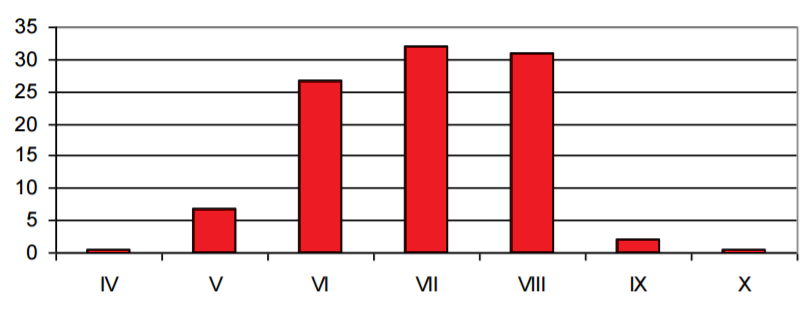
\includegraphics[scale=0.8]{./pictures/r_factor_graph.png}
      \caption[Rozdělení faktoru R během vegetačního období]{Rozdělení
        faktoru R během vegetačního období [\%] dle
        \cite{janecek2012}}
      \label{fig:r_faktor_graph}
\end{figure}
Faktor C vyjadřuje poměr smyvu z pozemku chráněném
pěstovanou plodinou ku~smyvu na pozemku, jež je udržován jako úhor,
kypřený po každém dešti. Nejlepší metodou je zjištění struktury
plodin, osevních postupů a metodiky hospodaření od~zemědělského
subjektu užívajícího daný pozemek.

Pro určení vegetačního faktoru lze využít Protierozní
kalkulačku\cite{kalkulacka}, která po vybrání příslušného osevního
postupu zobrazí C faktor pro celé období postupu. Toto určení C faktoru vychází z následující tabulky \ref{osevni_c}.

\begin{table}[!h]
\begin{center}
\catcode`\-=12
    \noindent\begin{tabular}{|*{4}{c|}}
    \hline
    \bf Osevní postup & \bf Výrobní oblast - zaměření & \bf Plodiny & \bf C\\
\hline Standartní & Bramborářská - brambory & (je, br, op, oz, br, jj)	& 0,27\\
\hline Standartní & Bramborářská - chov skotu& (je, op, ks, ks, ov) &0,27\\
\hline Standartní & Bramborářská - tržní plodiny &(br, op, or, oz, jj)& 0,32\\
\hline Standartní & Kukuřičná - bez ŽV &(op, kz, jj, or, op)& 0,29\\
\hline Standartní & Kukuřičná - tržní plodiny &(kz, ks, op, jj)& 0,32\\
\hline Standartní & Obilnářská &(je, op, jj, ks, op, br, jj)& 0,50\\
\hline Standartní & Obilnářská - obiloviny &(hr, op, jj, or, op, jj)& 0,29\\
\hline Standartní & Obilnářská - tržní plodiny &(je, oz, br, jj)& 0,23\\
\hline Standartní & Pícninářská &(jt, jt, br, jj, ov)&  0,17\\
\hline Standartní & Pícninářská &(jt, jt, jt, ov, br, jj)& 0,15\\
\hline Standartní & Řepařská - cukrovka & (cu, jj, hr, op) &0,11\\
\hline Standartní & Řepařská - tržní plodiny &(op, hr, or, op)& 0,27\\
\hline Ochranný & bez ŽV &(los, br, op, jj, hr, op)& 0,20\\
\hline Ochranný & bez ŽV &(op, kz, jj, or, op)& 0,22\\
\hline Ochranný & produkce mléka & (jts, jts, op, ov, br, oz)& 0,33\\
\hline Ochranný & chov prasat a skotu & (jts, jts, op, br, los, oj)& 0,18\\
\hline Ochranný & chov prasat & (jts, op, los, hr, oj)& 0,17\\
\hline Ochranný &  pásma ochrany vod a CHKO &(je, op, jj, or, op, jj)& 0,17\\
\hline Ochranný &  pásma ochrany vod a CHKO &(jts, jts, jts, op, oz, ov)& 0,17\\
\hline Ochranný &  pásma ochrany vod a CHKO &(jts, op, oz, gps, jj) & 0,11\\
\hline Ochranný &  pásma ochrany vod a CHKO &(jts, or, op, jj, ov) & 0,16\\
\hline
    \end{tabular}\\
  \caption[Hodnoty C faktoru pro jednotlivé osevní postupy]{Hodnoty C faktoru pro jednotlivé osevní postupy dle metodiky\cite{janecek2012}.}
  \label{osevni_c}
\end{center}
\end{table}
\FloatBarrier
\subsection{Faktor protierozních opatření (P)}
Při využití agrotechnických metod protierozní ochrany, jako jsou
konturové obdělávání, pásové střídání plodin, hrázkování či
terasování, je snižován faktor P. Důležité ovšem je dodržet podmínky
maximálních délek a počtu pásů, jinak musí být volena základní hodnota
P faktoru, tedy $P=1$.

Přehled všech metod a hodnot P faktoru lze najít v USLE\cite{usle1978}
nebo Janečkově metodice\cite{janecek2012}.

\subsection{Přípustná průměrná dlouhodobá ztráta půdy ($G_P$)}
Dle vypočteného faktoru G lze rozdělit potenciální ohrožení půdy do 6
kategorií.\cite{vumop}

\begin{table}[!h]
\begin{center}
\catcode`\-=12
    \noindent\begin{tabular}{|*{3}{c|}} \hline \bf Kategorie & \bf
    $\bf G~(t\cdot ha^{-1}\cdot rok^{-1})$ & \bf Kategorie ohroženosti
    vodní erozí\\ \hline 1 & méně než 1,0 & velmi slabě
    ohrožená\\ \hline 2 & 1,1 - 2,0 & slabě ohrožená\\ \hline 3 & 2,1
    - 4,0 & středné ohrožená\\ \hline 4 & 4,1 - 8,0 & silně
    ohrožená\\ \hline 5 & 8,1 - 10,0 & velmi silně ohrožená\\ \hline 6
    & více než 10,1 & extrémně ohrožená\\ \hline
    \end{tabular}\\
  \caption[Rozdělení potenciální ohroženosti půdy]{Rozdělení
    potenciální ohroženosti půdy dle VÚMOP \cite{vumop}.}
  \label{tabulka_ohrozenost}
\end{center}
\end{table}
\FloatBarrier Pro dlouhodobé zachování výrobních, ale i nevýrobních,
funkcí půdy je definována přípustná průměrná roční ztráta, která by
neměla být překročena. Pokud k tomu na pozemku dojde, je třeba zvolit
účinnější protierozní postupy. Hodnota faktor dlouhodobé ztráty půdy
se odvíjí od hloubky půdy, tu lze kromě terénního měření určit rovněž
z 5. číslice kódu BPEJ.\cite{janecek2012}

Mělké půdy (čísla 5 a 6) je doporučeno zatravnit, případně
zalesnit. Kromě půd s kódem 8 a 9, pro které je třeba hloubku půdy
potřeba zjistit terénním průzkumem, je pro ostatní půdy přípustná
hodnota $G_P=4,0~t\cdot ha^{-1}\cdot rok^{-1}$.\cite{Novotny2014}

%!TEX ROOT=radek-novotny-bp-2017.tex
%%% ML: v teto kapitole obecne chybi zdroje, reference
%%% RN: Doplneny reference, jeste chybi u Grass doplnim
\chapter{Technologie}
\label{3-technologie}
Cílem této kapitoly je v krátkosti popsat technologie, jež byly
použity pro implementaci teoretických poznatků do softwarového
nástroje – zásuvného modulu pro QGIS.
\section[QGIS]{QGIS 
\includegraphics[scale=0.055]{./pictures/qgis.png} 
\footnote{http://www.qgis.org/}}
\label{qgis}
\begin{figure}[H]
    \centering 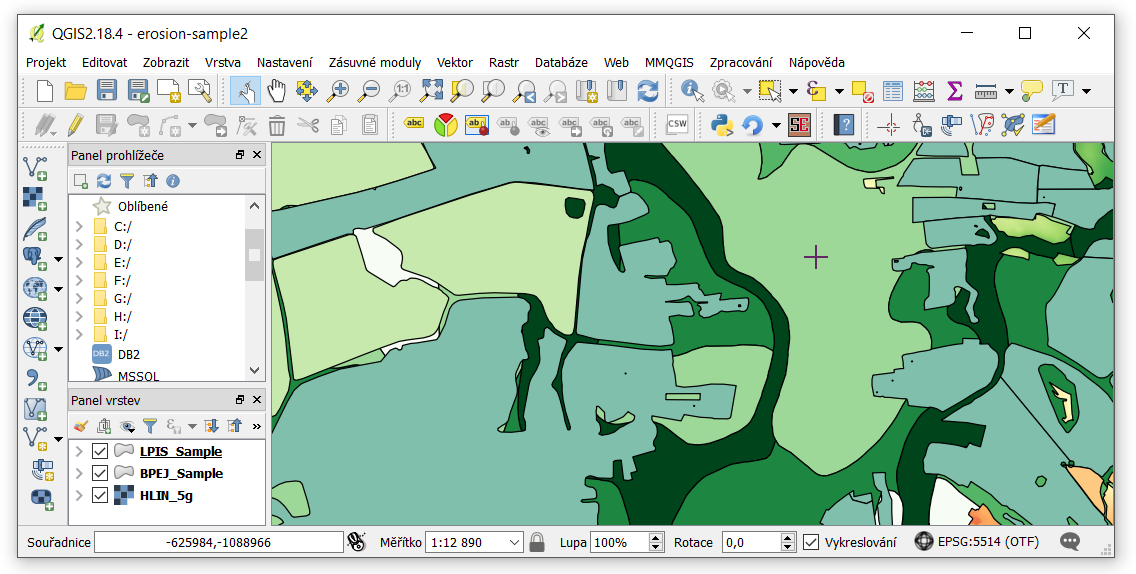
\includegraphics[scale=0.6]{./pictures/qgis_screen.png}
      \caption[Náhled prostředí QGIS 2.18]
      {Náhled prostředí QGIS 2.18, zdroj: autor}
      \label{screen:qgis}
\end{figure}
QGIS, jehož název vychází z původně používaného Quantum GIS, je open
source (licence GNU/GPL) geografický informační systém (GIS) dostupný
z platforem Mac OS X, Linux, Unix, a Microsoft Windows, přičemž od
roku 2014 je vyvíjena i verze pro Android. Samotný vývoj QGIS začal
Gary Sherman v roce 2002, poté byl projekt zařazen do Open Source
Geospatial Foundation (2007) a v roce 2009 vyšla jeho první verze. V
současnosti je aktuální verzí 2.18, jež by měla být poslední v druhé
řadě, přičemž by měla být nahrazena verzí 3.0, která bude postavena na
Python 3 s Qt5 a PyQt5. Od svého vzniku je QGIS udržován a dále
vyvíjen dobrovolníky.

QGIS podporuje většinu funkcí, které jsou od GIS očekávány, ať už se
jedná o podporu mnoha vstupních formátů vektorových i rastrových dat,
výběr a úpravy objektů nebo práci s atributovými tabulkami. Výhodou je
rovněž podpora nástrojů GRASS GIS, pomocí kterých jsou zvládány
složitější výpočetní operace.  Silnou stránkou jsou rovněž zásuvné
moduly (pluginy). Díky rozsáhlé uživatelské komunitě v akademickém,
ale stále častěji i profesním prostředí, a veřejné licenci GNU/GPL,
pod kterou celý QGIS funguje, je vývoj nových zásuvných modulů značně
zjednodušen. V QGIS je pluginů velké množství, čímž se významně
rozšiřují možnosti práce se softwarem. Zásuvný modul pro QGIS je i
výsledkem této práce.\cite{masteringQgis}
\section[GRASS GIS]{GRASS GIS 
\includegraphics[scale=0.12]
{./pictures/grass.png} \footnote{https://grass.osgeo.org/download/logos/}}
\label{grassgis}
\begin{figure}[H]
    \centering 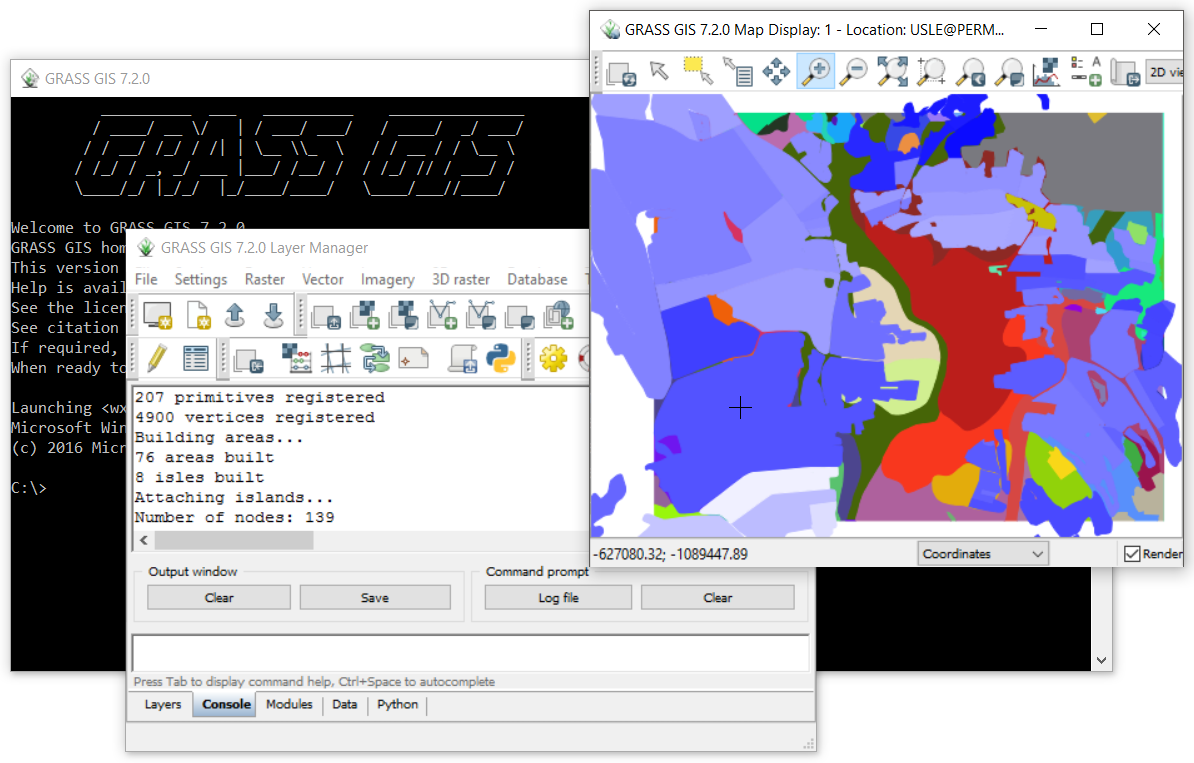
\includegraphics[scale=0.6]{./pictures/grass_screen.png}
      \caption[Náhled prostředí GRASS GIS 7.2.0]
      {Náhled prostředí GRASS GIS 7.2.0, zdroj: autor}
      \label{screen:grass}
\end{figure}
GRASS GIS (Geographic Resources Analysis Support System) je stejně
jako QGIS multiplatformním geografickým informačním systémem, který je
volně šiřitelný pod licencí GNU/GPL. Jeho vývoj započala U.S. Army
Corps of Enginneer/CERL (Construction Engineering Research Lab) už
počátkem 80. let, na jejich konci byly veškeré zdrojové kódy uvolněny
veřejnosti a v roce 1995 CERL z projektu odešel úplně. Další vývoj se
poté začal odehrávat na akademické půdě, především na Baylor
University v Texasu, USA a v Hannoveru v Německu. V roce 2008 byl
projekt zařazen do Open Source Geospatial Foundation.

GRASS pracuje s vektorovými i rastrovými daty pomocí modulů, kterých
je z obdobných důvodů jako u QGIS mnoho. Technika použití modulů je
spjata s dlouhou historií a počátky vývoje softwaru, kdy bylo potřeba
s výkonem procesoru i využitím operační paměti šetřit.

Dalším specifikem GRASS GIS je nutnost pracovat s daty v pevně
definované adresářové struktuře, díky čemuž je uživatel nucen data
systematizovat. Struktura je rozdělena na databázi, lokaci a mapset.
%%% ML: k pomlckach, tady chcete vyctove prostredi (itemize/enumerate)?
%%% RN: ano, text nebyl v dobe kontroly finalne upraven, opraveno
\begin{itemize}
	\item \textbf{Databáze} (Databanka) je běžným adresářem na disku a 
	obsahuje veškerá data, ke kterým GRASS přistupuje.
	\item \textbf{Lokace} (Projekt) je adresář umístěný v databance, 
	pro který je definován souřadnicový systém a jeho obsahem jsou data 
	související s daným projektem.
	\item \textbf{Mapset} tvoří soubor map z jedné lokace, jež jsou 
	určitým způsobem logicky provázány. Součástí každé lokace je mapset 
	s názvem PERMANENT, který by měl obsahovat základní datové vrstvy.
\end{itemize}
GRASS je možné ovládat, jak z příkazové řádky, tak pomocí GUI. Další
možností je přistupovat k modulům GRASS pomocí GUI QGIS, které mnoho
uživatelů shledává přívětivějším.
\newpage
\section[Python]{Python 
\includegraphics[scale=0.2]{./pictures/python.png}
\footnote{https://www.python.org/community/logos/}}
\label{python}
Celý kód byl psán ve skriptovacím programovacím jazyce Python. Jedná
se o objektově orientovaný jazyk představený v roce 1991 Guido van
Rossumem. Python je dále vyvíjen jako open source projekt, který je
zdarma distribuován na většinu platforem. Jazyk se vyznačuje
jednoduchou, ale účelnou syntaxí, reprezentovanou např. dynamickou
kontrolou datových typů nebo definicí bloků pomocí odsazování. Výhodou
Pythonu je i jeho poměrně snadné rozšíření jazykem C, který je
výkonnější a dokáže zrychlit náročnější operace.

V současné době je stále nejvyužívanější verzí Python 2.7.x, kterou
byla druhá řada ukončena a nyní se v ní jen opravují chyby. Už od roku
2008 je ve vývoji třetí řada, ta však není zpětně kompatibilní. Proto
%%% ML: co to zname pro vas kod?
%%% RN: doplneno
je potřeba software napsaný v Python 2 pro novou verzi adaptovat. Kód 
pluginu vyvíjeného v této práci byl již vytvářen s ohledem na novou 
verzi Python 3 a měl by být kompatibilní s oběma verzemi.
\cite{diveIntoPython}\cite{learningPython}

\section[PyCharm]{Pycharm 
\includegraphics[scale=0.2]
{./pictures/pycharm.png} \footnote{https://www.jetbrains.com/pycharm/}}
\label{python}
\vspace{-10pt}
\begin{figure}[H]
    \centering 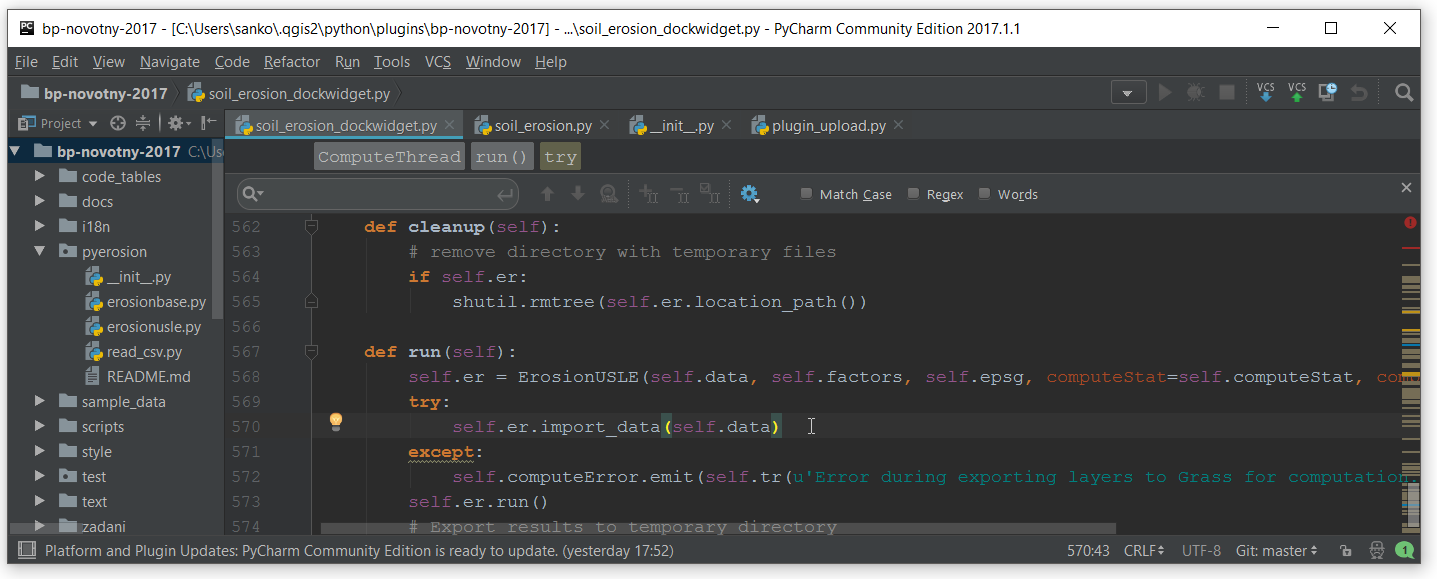
\includegraphics[scale=0.45]{./pictures/pycharm_screen.png}
      \caption[Náhled vývojového prostředí PyCharm]{Náhled vývojového 
      prostředí PyCharm, zdroj: autor}
      \label{screen:pycharm}
\end{figure}
\vspace{-10pt}
Pro vývoj zdrojového kódu bylo využito vývojové prostředí(IDE - 
Integrated Development Environment)  PyCharm, který byl vyvinut 
českou společností JetBrains. Toto prostředí bylo vytvořeno primárně 
pro Python a pro open source projekty je zdarma. Jeho výhodami jsou 
automatické doplňování textu, hledání syntaktických chyb či vytváření 
oddělených projektů. Osobně oceňuji zejména přehlednost a rychlost 
psaní kódu v tomto IDE.\cite{masteringPycharm}
\section[GitHub]{GitHub 
\includegraphics[scale=0.06]{./pictures/github.png} 
\footnote{https://github.com/}}
\label{github}
\begin{figure}[H]
    \centering 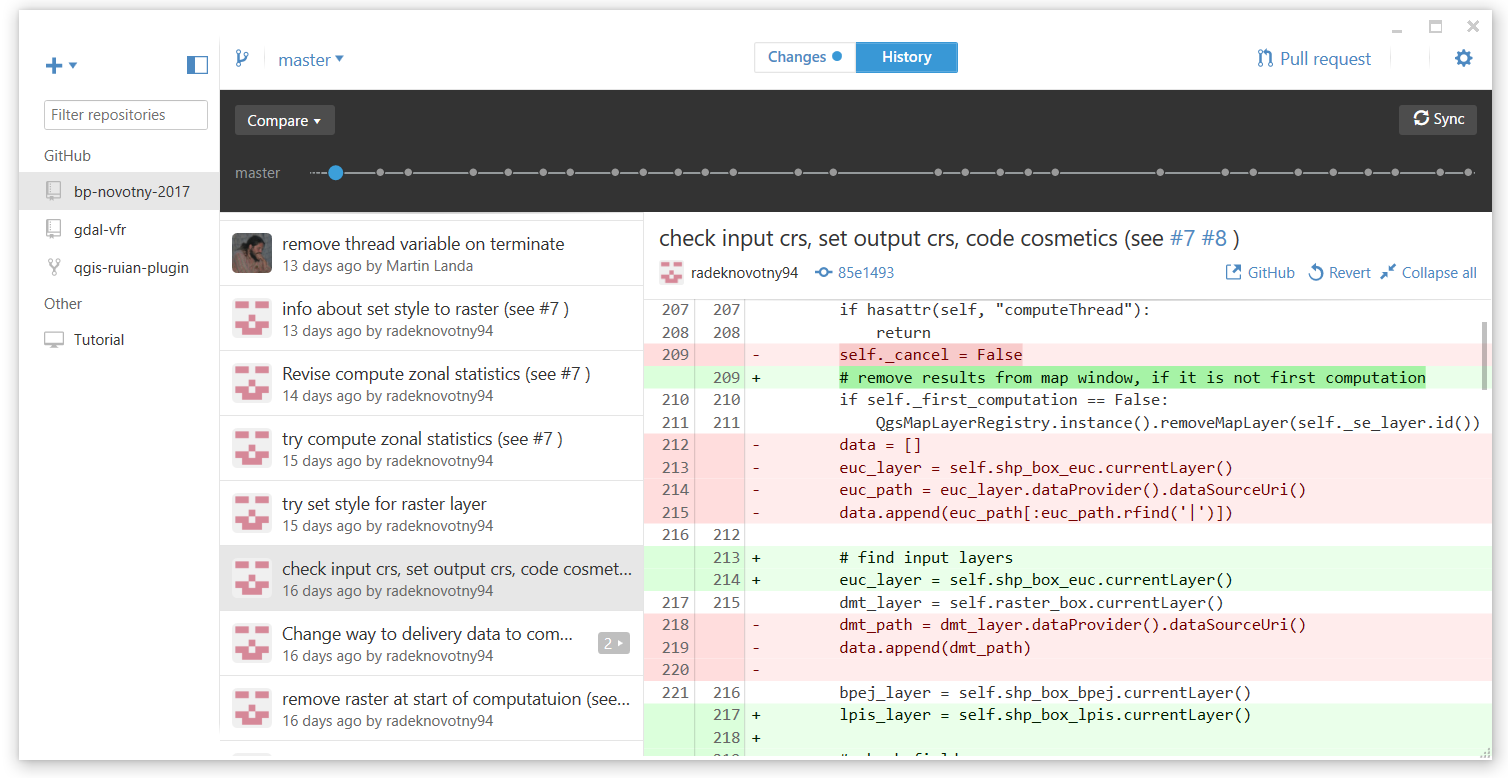
\includegraphics[scale=0.45]{./pictures/github_screen.png}
      \caption[Náhled verzovacího prostředí GitHub]
      {Náhled verzovacího prostředí GitHub, zdroj: autor}
      \label{screen:github}
\end{figure}
GitHub je webová služba podporující verzovací nástroj Git, což je distribuovaný (kolektivní) systém správy verzí. Git byl vytvořen Linusem Torvaldsem pro vývoj jádra operačního systému Linux a funguje pod licencí GNU/GPL. Na tomto základu je tedy postaven GitHub, který pro open source projekty zdarma nabízí vytvoření repositáře se zdrojovým kódem, dokumentací, historií verzování, systémem pro sledování problémů (Issue tracking), zobrazování rozdílů mezi verzemi a mnoho dalšího.\cite{introducingGithub}

\section[Qt]{Qt 
\includegraphics[scale=0.20]{./pictures/qt.png} 
\footnote{https://www.qt.io/ide/}}
\label{qt}
\begin{figure}[H]
    \centering 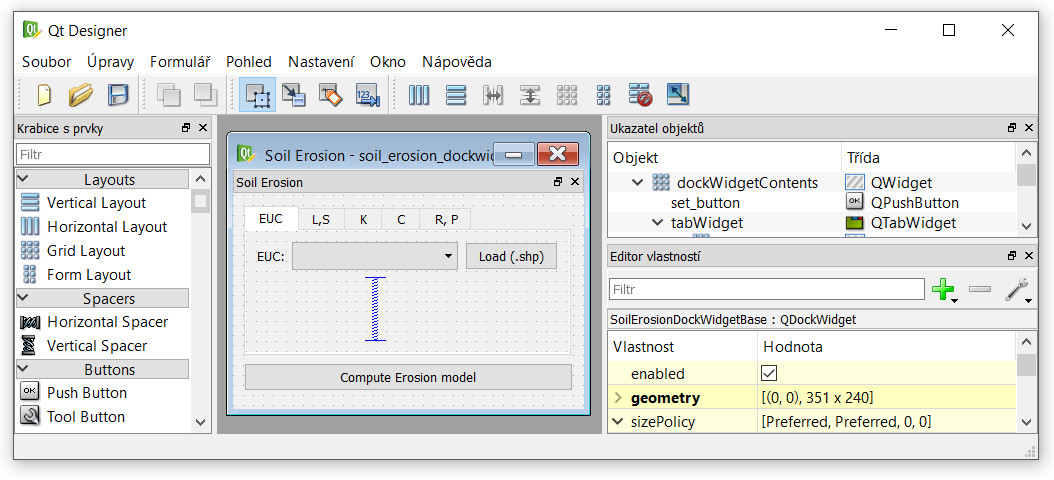
\includegraphics[scale=0.6]{./pictures/qt_screen.png}
      \caption[Náhled prostředí Qt Designer]
      {Náhled prostředí Qt Designer, zdroj: autor}
      \label{screen:qt}
\end{figure}
Qt je multiplatformní aplikační framework, který je využíván pro
tvorbu aplikací s grafickým uživatelským rozhraním (GUI). Qt toolkit
byl vytvořen v roce 1999 firmou Trolltech, v roce 2008 jej odkoupila
společnost Nokia, která je stále hlavním vývojářem toolkitu, přestože
v roce 2011 prodala licenci na komerční projekty vytvořené v Qt firmě
Digia.

Hlavními aplikacemi jsou Qt Creator, sloužící ke kompletní tvorbě
aplikací, a Qt Designer, pomocí kterého je navrhováno samotné
GUI. Výhodou je přizpůsobení výsledného GUI nativnímu vzhledu
operačního systému. Qt podporuje používání řady jazyků, od výchozího
C++ po Python, který je na Qt navázán pomocí frameworku PyQt.\cite{qt}
\cite{rapidPyQt}


% Vysázení seznamu zkratek
\begin{seznamzkratek}{ABCDE}
	\novazkratka{bpej}
	      {BPEJ}
	      {Bonitovaná půdně ekologická jednotka}

    \novazkratka{bpv}
	      {Bpv}
	      {Balt po vyrovnání}

    \novazkratka{cuzk}
	      {ČÚZK}
	      {Český úřad zeměměřičský a katastrální}

    \novazkratka{dmr}
	      {DMR}
	      {Digitální model reliéfu}

    \novazkratka{dmt}
	      {DMT}
	      {Digitální model terénu}

    \novazkratka{euc}
	      {EUC}
	      {Erozně uzavřený celek}

	\novazkratka{gis}
	      {GIS}
	      {Geografický informační systém (Geographic information system)}	

	\novazkratka{hpj}
	      {HPJ}
	      {Hlavní půdní jednotka}	

	\novazkratka{lpis}
	      {LPIS}
	      {Registr půdy (Land Parcel Identification System)}

	\novazkratka{musle}
	      {MUSLE}
	      {Modifikovaná univerzální rovnice ztráty půdy (Modified universal Soil Loss Equation)}

	\novazkratka{rusle}
	      {RUSLE}
	      {Revidovaná univerzální rovnice ztráty půdy (Revised universal Soil Loss Equation)}

    \novazkratka{tin}
	      {TIN}
	      {nepravidelná trojúhelníková síť (Triangulated Irregular Network)}

	\novazkratka{usle}
	      {USLE}
	      {Univerzální rovnice ztráty půdy (Universal Soil Loss Equation)}

	\novazkratka{vumop}
	      {VÚMOP}
	      {Výzkumný ústav meliorací a ochrany půdy, v.v.i.}

\end{seznamzkratek}

% Literatura
\nocite{*}
\def\refname{Literatura}
\bibliographystyle{mystyle}
\bibliography{radek-novotny-bp-2017-literatura}


% Začátek příloh
%\def\figurename{Figure}%
%\prilohy

% Vysázení seznamu příloh
%\seznampriloh

% Vložení souboru s přílohami
%%!TEX ROOT=radek-novotny-bp-2017.tex
\chapter{Uživatelský manuál}
\label{6-manual}
\section{O pluginu Soil Erosion}
\label{o_pluginu} Zásuvný modul Soil Erosion slouží pro výpočet a
prezentaci erozního smyvu na orné půdě.

Vstupem jsou vektorové vrstvy Bonitovaných půdně ekologických jednotek
(BPEJ)\footnote{\url{http://www.spucr.cz/bpej/celostatni-databaze-bpej}},
Registru půd
(LPIS)\footnote{\url{http://eagri.cz/public/app/eagriapp/lpisdata/}} a
rastrová vrstva digitálního modelu terénu.

Výstupem je rastrová vrstva znázorňující lokální hodnotu smyvu a
vektorová vrstva obsahující výsledné hodnoty průměrné dlouhodobé
ztráty půdy pro definované erozně uzavřené celky.

Zásuvný modul je pod licencí GNU/GPL.

Případné chyby a nápady na vylepšení zásuvného modulu prosím pište na
stránku
pluginu\footnote{\url{https://github.com/ctu-geoforall-lab-projects/bp-novotny-2017/issues}}.

\section{Instalace}
\label{manual_instalace} Zásuvný modul \textit{Soil Erosion} je v
současnosti veden jako \uv{Experimentální} a není zařazen do
oficiálního repositáře QGIS. Jedinou odlišností od instalace jiných
zásuvných modulů je nutnost přidání repositáře laboratoře
\textit{CTU GeoForAll Lab}, ve kterém je plugin \textit{Soil Erosion}
umístěn.


\subsection{Přídání repositáře \textit{CTU GeoForAll Lab}} \textit{Zásuvné
moduly} $\rightarrow$ \textit{Spravovat a instalovat zásuvné
moduly...}.

	\begin{figure}[H] \centering
		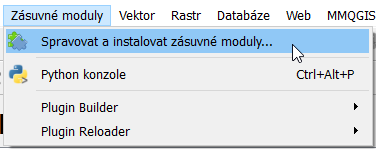
\includegraphics[width=.6\textwidth]{./pictures/otevreni_okna_zasuvne_moduly.png}
		\caption[Otevření okna \textit{Zásuvné
moduly}]{Otevření okna \textit{Zásuvné moduly}, zdroj: autor}
		\label{fig:manual_otevreni_okna_zasuvne_moduly}
 	\end{figure}
 	
V záložce \textit{Nastavení} zkontrolujte, zda je volba
\textit{Zobrazit také experimentální zásuvné moduly} aktivní.

Kliknutím na tlačítko \textit{Přidat...} připojíme repositář
laboratoře \textit{CTU GeoForAll
Lab}\footnote{\url{http://geomatics.fsv.cvut.cz/research/geoforall}}

\begin{lstlisting}[basicstyle=\footnotesize\ttfamily, backgroundcolor
= \color{light-gray}, numbers=left, columns=fullflexible,
keepspaces=true] Nazev: CVUT GeoForAll Lab URL:
http://geo.fsv.cvut.cz/geoforall/qgis-plugins.xml
\end{lstlisting}

	\begin{figure}[H] \centering
		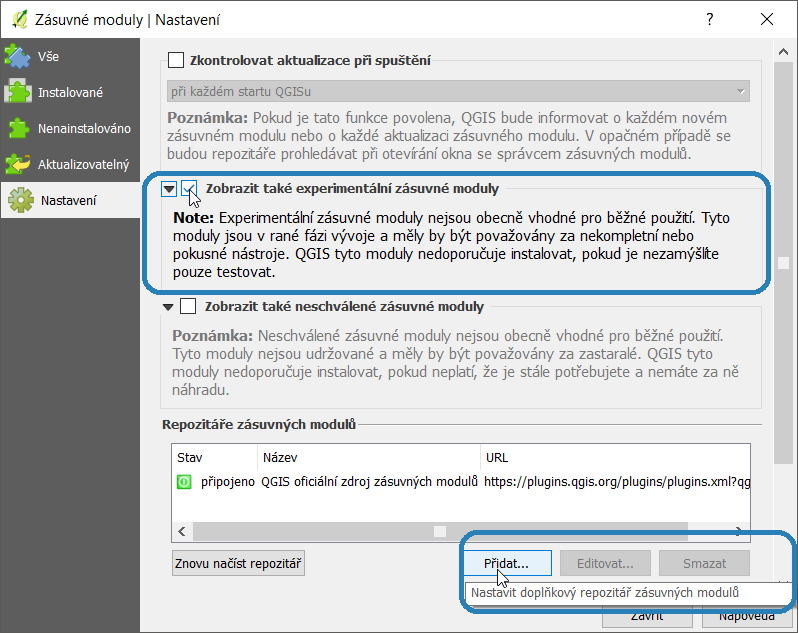
\includegraphics[width=.85\textwidth]{./pictures/pridani_repositare.png}
		\caption[Aktivování experimentálních zásuvných modulů
a přidání repositáře.]{Aktivování experimentálních zásuvných modulů a
přidání repositáře, zdroj: autor}
		\label{manual_pridani_repozitare}
 	\end{figure}
 	
	\begin{figure}[H] \centering
		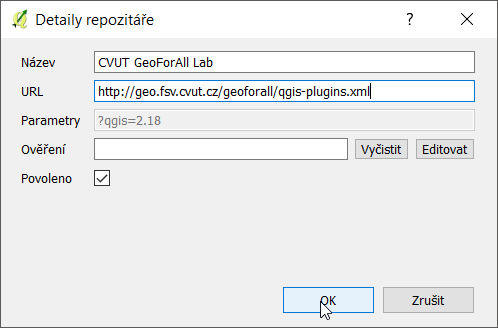
\includegraphics[width=.6\textwidth]{./pictures/zadani_repositare.png}
		\caption[Přidání repositáře GeoForAll Lab]{Přidání
repositáře CTU GeoForAll Lab, zdroj: autor}
		\label{manual_zadani_repozitare_geoforall_lab}
 	\end{figure}

\subsection{Instalace zásuvného modulu \textit{Soil Erosion}} Po
připojení repositáře vyhledejte \textit{Soil Erosion Plugin}, buďto v
záložce \textit{Vše} nebo \textit{Nenainstalované}. Po výběru
zásuvného modulu klikněte na \textit{Instalovat zásuvný modul}.

	\begin{figure}[H] \centering
		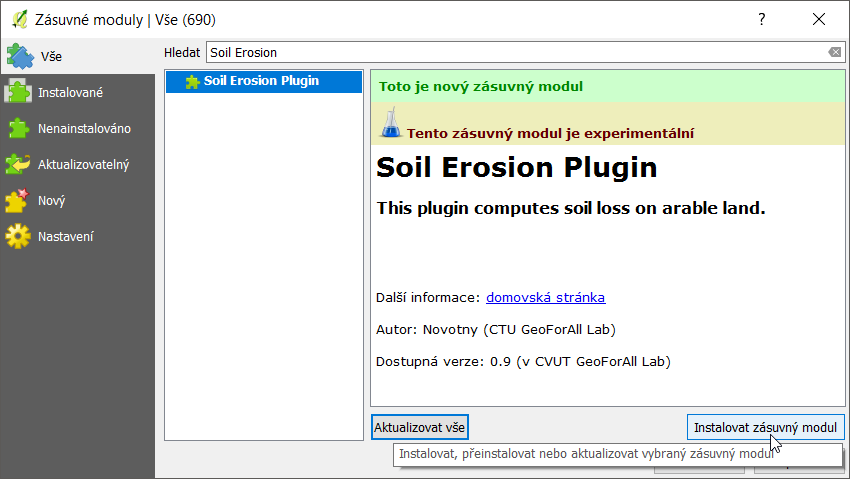
\includegraphics[width=.8\textwidth]{./pictures/instalace_pluginu.png}
		\caption[Instalace zásuvného modulu]{Instalace
zásuvného modulu, zdroj: autor}
		\label{fig:manual_pridani_repozitare_geoforall_lab}
 	\end{figure}
	
Po úspěšném nainstalování se v \textit{Panelu nástrojů Zásuvné moduly}
objeví jeho ikona. Zásuvný modul je možné spustit kliknutím na jeho
ikonu nebo z menu \textit{Zásuvné moduly} $\rightarrow$ \textit{Soil
Erosion} $\rightarrow$ \textit{Soil Erosion Plugin}.
	
	\begin{figure}[H] \centering
		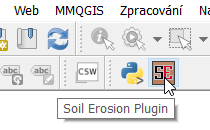
\includegraphics[width=.3\textwidth]{./pictures/spusteni_pluginu2.png}
		\caption[Ikona zásuvného modulu v panelu
nástrojů]{Ikona zásuvného modulu v panelu nástrojů, zdroj: autor}
		\label{ikona_modulu_v_panelu_nastroju}
 	\end{figure}
	
	\begin{figure}[H] \centering
		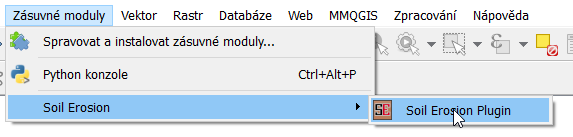
\includegraphics[width=.7\textwidth]{./pictures/spusteni_pluginu1.png}
		\caption[Ikona zásuvného modulu v menu]{Ikona
zásuvného modulu v menu, zdroj: autor}
		\label{ikona_modulu_v_panelu_nastroju2}
 	\end{figure}

\section{Návod k použití}
\label{navod_k_pouziti} Pro vytvoření erozního modelu je nutné
vyplnění pěti záložek, ve kterých jsou definovány pozemky, na kterých
bude výpočet probíhat (EUC), a voleny vstupy pro určení faktorů v
rovnici USLE (LS, K, C a RP).
\subsection{EUC} Určení erozně uzavřených celků (pozemků), pro které
bude určována průměrná roční ztráta, probíhá v záložce EUC.

	\begin{figure}[H] \centering
		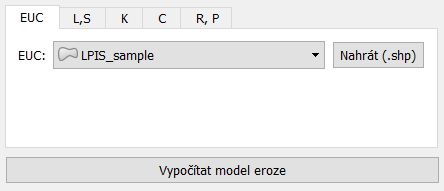
\includegraphics[width=.5\textwidth]{./pictures/euc.png}
		\caption[Záložka EUC]{Záložka EUC, zdroj: autor}
		\label{zalozka_euc}
 	\end{figure}

Zde se volí polygonová vektorová vrstva (.shp) definující EUC. Vrstvu
je možné zvolit ze seznamu vrstev, či ji nahrát přes tlačítko
\textit{Nahrát (.shp)}.

Tato vrstva většinou vychází z vrstvy LPIS, ovšem je rovněž možné
volit svou vlastní vrstvu. Ovšem při zvolení vlastní vrstvy je potřeba
dát pozor, aby na většině plochy EUC byly definovány faktory K a C.

\paragraph{Poznámka:} Při využítí vrstvy LPIS je pro správnou
funkčnost výpočtu doporučeno zkontrolovat návaznosti polygonů. Zda v
místech, kde se jedná o jeden EUC rozdělený mezi několik vlastníků
(uživatelů), na sebe polygony navazují (případně se překrývají). (EUC
1A a EUC 1B)

Naopak v místech, kde jsou pozemky erozně odděleny technické
protierozním opatření či silnicí, musí být mezi jednotlivými polygony
mezera. (EUC 2 a EUC 3)
\begin{figure}[H] \centering
		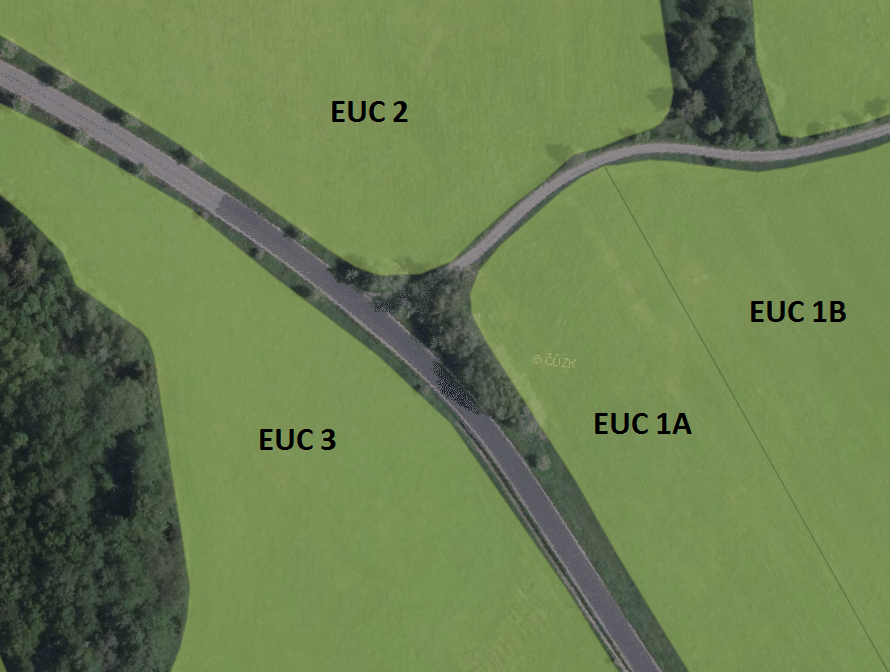
\includegraphics[width=.7\textwidth]{./pictures/rozdeleni_euc.png}
		\caption[Zobrazení EUC se zahrnutými
překážkami]{Zobrazení EUC se zahrnutými překážkami, zdroj: autor}
		\label{rozdeleni_euc}
\end{figure} Pro základní kontrolu je vhodné využití ortofota.
\subsection{L,S} V záložce L,S se určuje rastr digitálního modelu
terénu, nad kterým bude probíhat výpočet faktorů délky a sklonu svahu
(L, S). Vrstvu je možné zvolit ze seznamu vrstev, či ji nahrát přes
tlačítko \textit{Nahrát (rastr)}.
\begin{figure}[H] \centering
		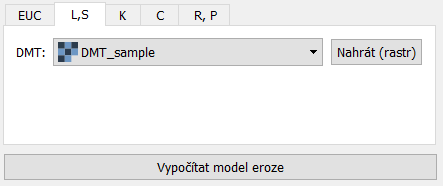
\includegraphics[width=.6\textwidth]{./pictures/ls.png}
		\caption[Záložka L,S]{Záložka L,S, zdroj: autor}
		\label{zalozka_ls}
\end{figure}
\subsection{K} V záložce K se volí polygonová vektorová vrstva (.shp)
BPEJ. Vrstva musí obsahovat pole s názvem \uv{BPEJ} ve formátu
\uv{X.XX.XX}, ze kterého se pomocí tlačítka \textit{Vypočítat K
faktor}, vypočte hodnota K a vrstva se dle jeho hodnoty barevně
rozliší. Případně je možné použít vrstvu s předem vypočteným K
faktorem v poli \textit{K}. Vrstvu je možné zvolit ze seznamu vrstev,
či ji nahrát přes tlačítko \textit{Nahrát (.shp)}.
\begin{figure}[H] \centering
		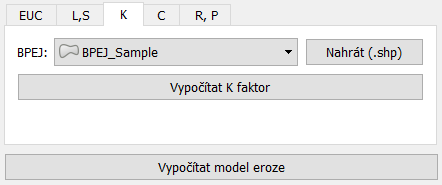
\includegraphics[width=.6\textwidth]{./pictures/k.png}
		\caption[Záložka K]{Záložka K, zdroj: autor}
		\label{zalozka_k}
\end{figure}
\paragraph{Tip:} Hodnoty K lze poté manuálně upravovat v atributové
tabulce (stejně lze upravovat i hodnoty C)
\subsection{C} Záložka C slouží ke zvolení polygonové vektorové vrstvy
(.shp) LPIS. Vrstva musí obsahovat pole s názvem \uv{KULTURAKOD} s
jednoznakovým kódem pro využití pozemku. V rolovací nabídce se volí
primární osevní postup užívaný na pozemcích s ornou půdou. Poté se C
faktor nastaví kliknutím na tlačítko \textit{Vypočítat C faktor},
přičemž současně dojde k barevnému rozlišení dle využití pozemku.
\begin{figure}[H] \centering
		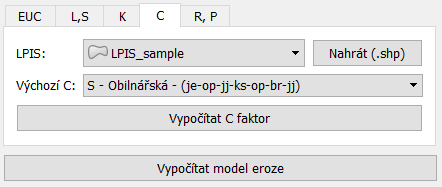
\includegraphics[width=.6\textwidth]{./pictures/c.png}
		\caption[Záložka C]{Záložka C, zdroj: autor}
		\label{zalozka_c}
\end{figure}
\paragraph{Poznámka:} Při využití dat LPIS vyexportovaných z Registru
půd
(LPIS)\footnote{\url{http://eagri.cz/public/app/eagriapp/lpisdata/}}
a~BPEJ\footnote{\url{http://www.spucr.cz/bpej/celostatni-databaze-bpej}}
z celostátní databáze, jejich formát odpovídá požadavkům zásuvného
modulu.
\paragraph{Tip:} Hodnoty C lze poté manuálně upravovat v atributové
tabulce (stejně lze upravovat i hodnoty K)
\subsection{R,P} V poslední záložce \textit{R,P} je možné upravit
hodnotu faktoru přívalového deště \textit{R} pro danou oblast. Tato
hodnota je nastavena na 40, což je průměrná hodnota pro ČR. Dále pak
hodnotu faktoru protierozních opatření \textit{P}, ta je nastavena na
1 (= Nejsou použita žádná agrotechnická protierozní opatření.)
\begin{figure}[H] \centering
		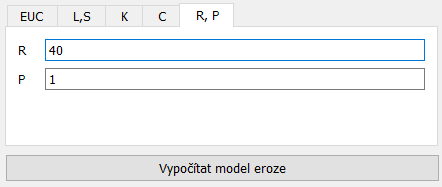
\includegraphics[width=.55\textwidth]{./pictures/rp.png}
		\caption[Záložka RP]{Záložka RP, zdroj: autor}
		\label{zalozka_rp}
\end{figure}
\subsection{Výpočet erozního modelu} Po nastavení všech vstupních
hodnot se stisknutím tlačítka provede výpočet erozního
modelu. Tlačítko je viditelné ze všech záložek. Po spuštění výpočtu
jsou zobrazovány informace o jeho průběhu pomocí panelu v horní části
QGIS. Z tohoto panelu je také možné výpočet ukončit pomocí tlačítka
\textit{Zrušit výpočet}.
\begin{figure}[H] \centering
		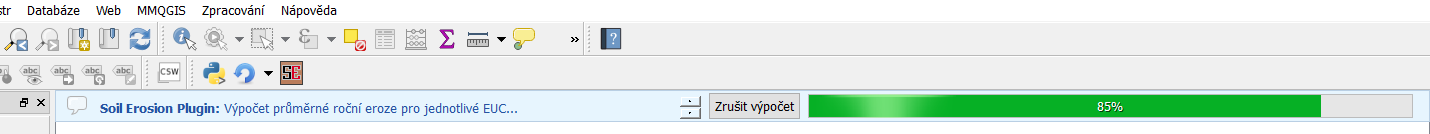
\includegraphics[width=.9\textwidth]{./pictures/progressbar.png}
		\caption[Informačního panel]{Informační panel,
zdroj: autor}
		\label{informacni_panel}
\end{figure}
\subsection{Erozní model} Po skončení výpočtu se do mapového okna na
první a druhé místo v seznamu vrstev přidají vrstvy erozního modelu -
\textit{EUC} a \textit{Lokální eroze}. Ukázku těchto vrstev je možné
najít v popisu ukázkového výpočtu.
\begin{itemize}
	\item Erozní model: Vektorová polygonová vrstva \textit{EUC}
je vytvořená z vrstvy zadané v záložce EUC. Do atributové tabulky této
vrstvy je přidán nový sloupec G s hodnotou průměrné roční ztráty půdy
pro jednotlivé pozemky, tyto pozemky jsou rovněž obarveny dle tabulky
ohrožení půdy.
	\item G faktor: Rastrová vrstva zobrazující lokální hodnoty
eroze ve stupních šedi.
\end{itemize} Při spuštění nového výpočtu se vytvořené vrstvy nahradí
novými.

\section{Ukázkový výpočet}

\subsection{Vzorová data} Pro ukázkový výpočet jsou použita vzorová
data. Ta obsahují 3 vrstvy \textit{DMT\_sample}, \textit{BPEJ\_Sample}
a \textit{LPIS\_Sample}.
%%% ML: chybi odkaz na testovaci data umistena v Git repozitari
\begin{figure}[H] \centering
		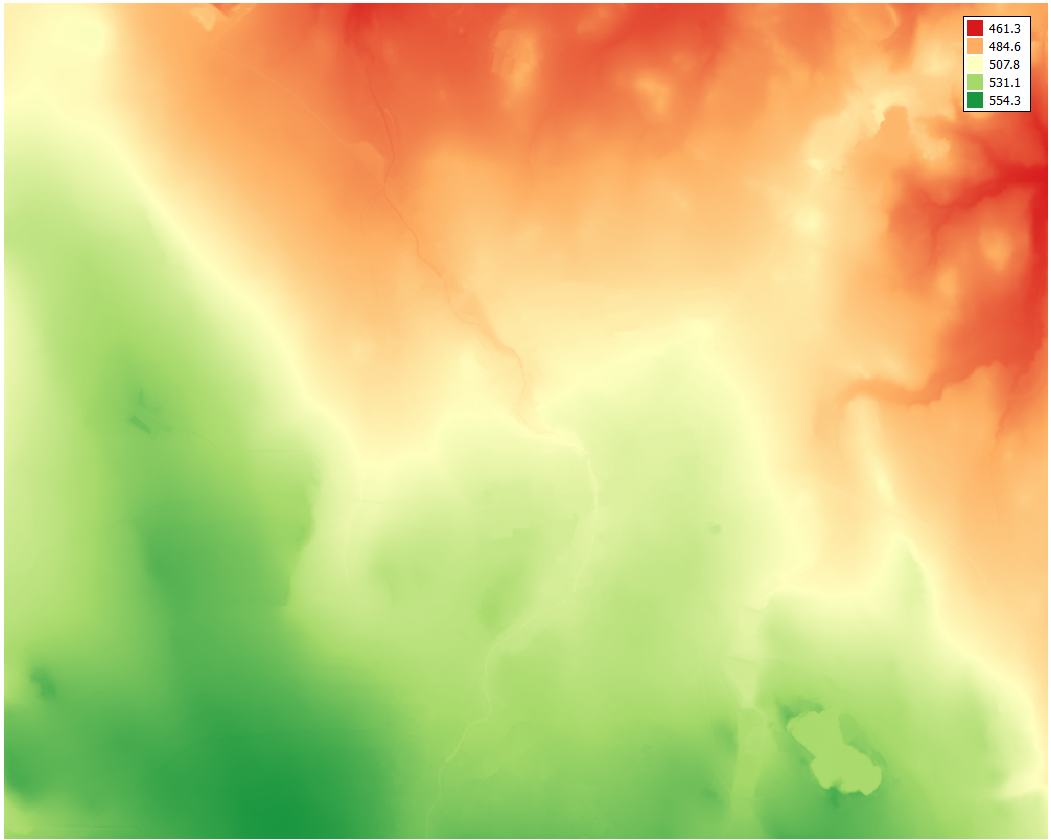
\includegraphics[width=.4\textwidth]{./pictures/dmt_layer1.png}
		\caption[Vrstva DMT\_sample]{Vrstva DMT\_sample,
zdroj: autor}
		\label{dmt_sample}
\end{figure}
\begin{figure}[H] \centering
		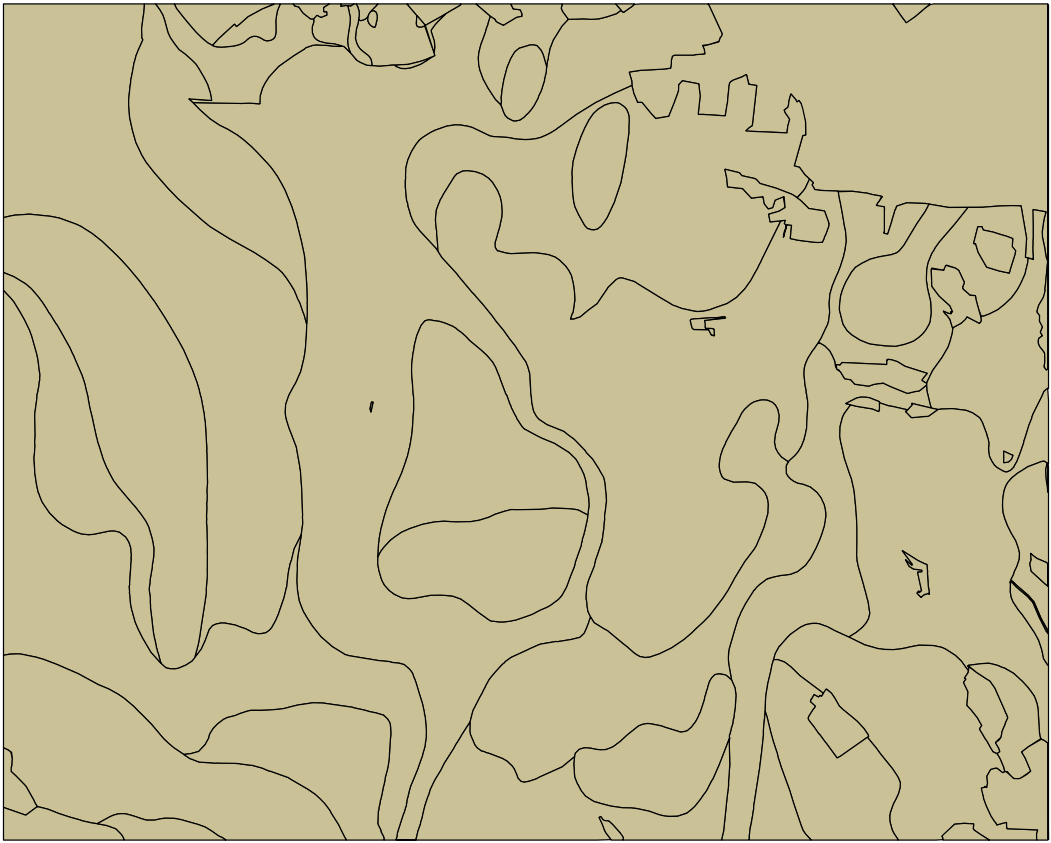
\includegraphics[width=.4\textwidth]{./pictures/bpej_layer1.png}
		\caption[Vrstva BPEJ\_sample]{Vrstva BPEJ\_sample,
zdroj: autor}
		\label{bpej_sample}
\end{figure}
\begin{figure}[H] \centering
		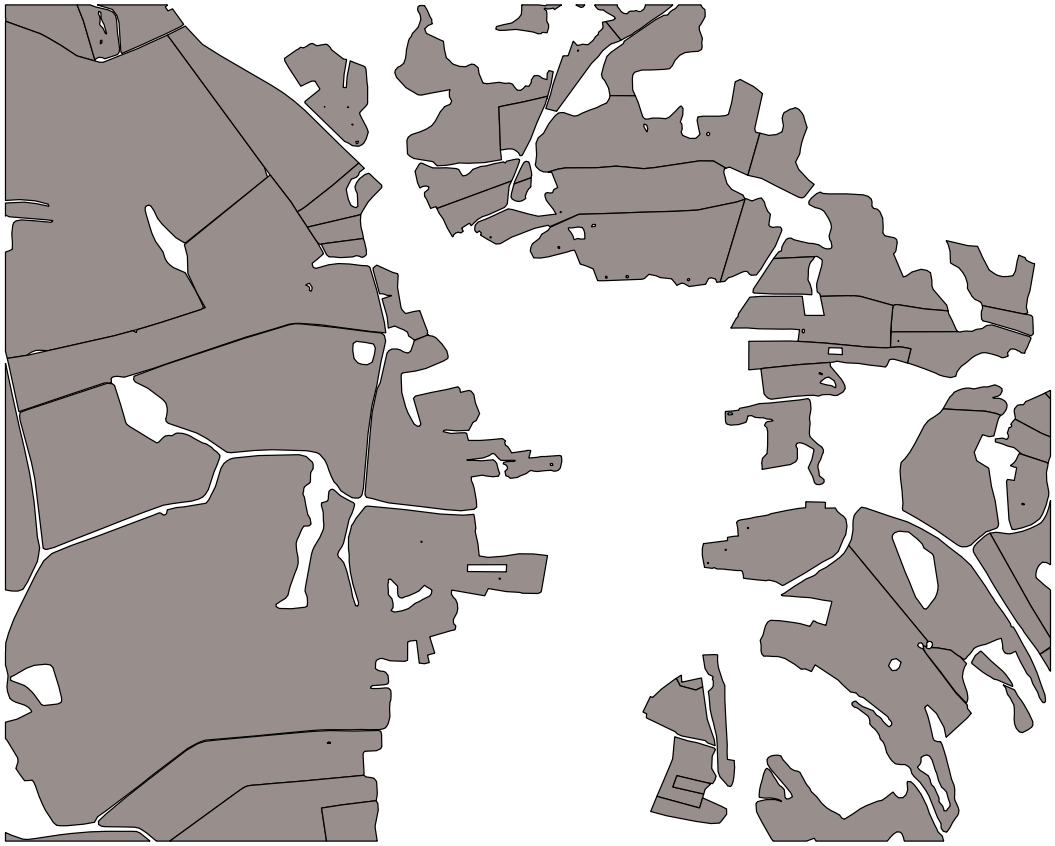
\includegraphics[width=.4\textwidth]{./pictures/lpis_layer1.png}
		\caption[Vrstva LPIS\_sample]{Vrstva LPIS\_sample,
zdroj: autor}
		\label{lpis_sample}
\end{figure}
\subsection{Nastavení vstupů a výpočet} Nastavení vstupních hodnot se
provede podle obecného návodu, kdy se jako EUC vrstva zvolí
%%% ML: nebavili jsme se o tom, ze se vrtsva EUC bude mirne od LPIS
%%% lisit? (tak jak to mate popsano v textu)
LPIS\_sample, v následujících záložkách názvy požadovaných vrstev
odpovídají jménu vzorových dat. Po výpočtu faktorů K a C v daných
záložkách se vrstvy obarví.
\begin{figure}[H] \centering
		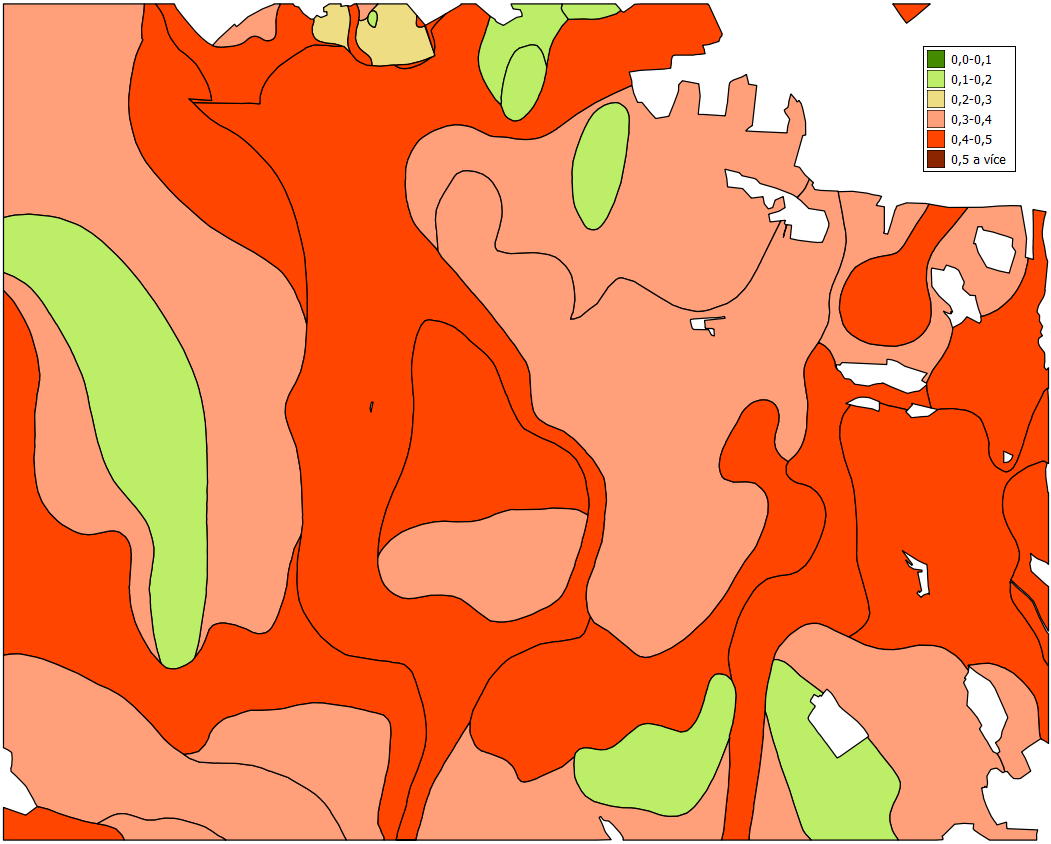
\includegraphics[width=.5\textwidth]{./pictures/bpej_layer2.png}
		\caption[Vrstva BPEJ\_sample po výpočtu K
faktoru]{Vrstva BPEJ\_sample po výpočtu K faktoru, zdroj: autor}
		\label{bpej_sample2}
\end{figure}
\begin{figure}[H] \centering
		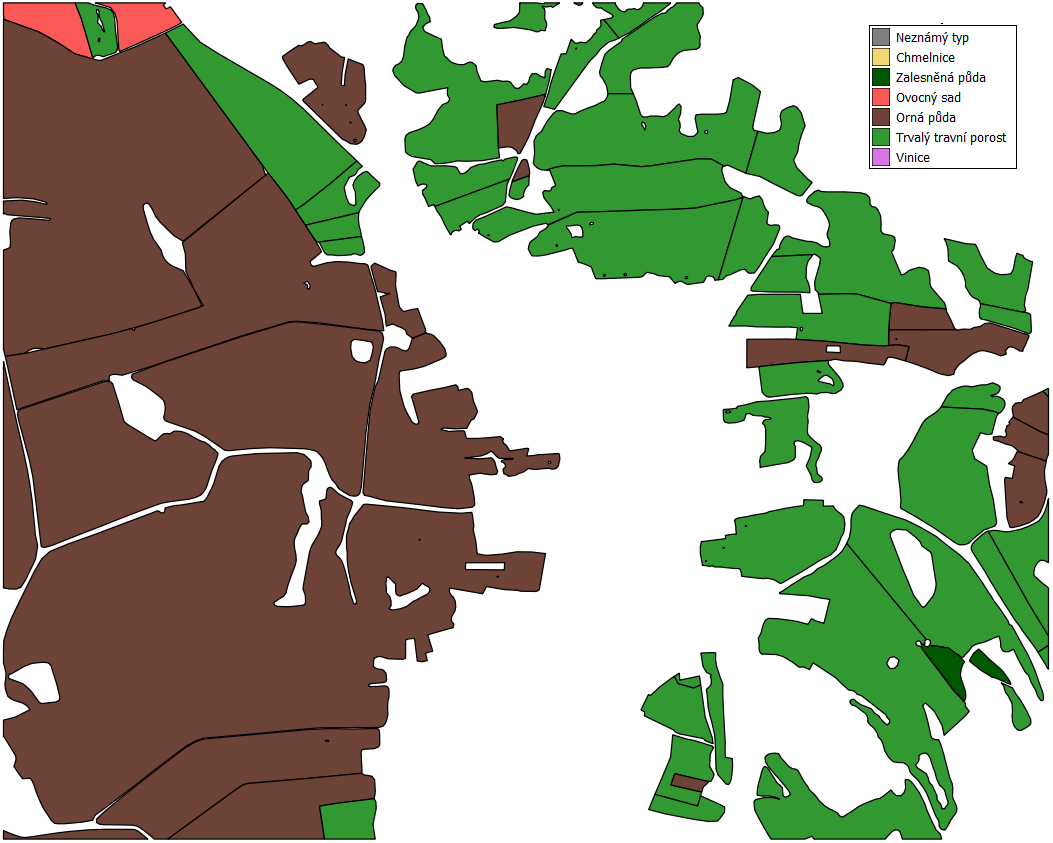
\includegraphics[width=.5\textwidth]{./pictures/lpis_layer2.png}
		\caption[Vrstva LPIS po výpočtu C faktoru]{Vrstva LPIS
po výpočtu C faktoru, zdroj: autor}
		\label{lpis_sample2}
\end{figure} V poslední záložce R,P jsou ponechány výchozí hodnoty a
plugin je spuštěn.
\newpage
\subsection{Výsledný model} Výsledkem výpočtu by měly být následující
vrstvy:
\begin{figure}[H] \centering
		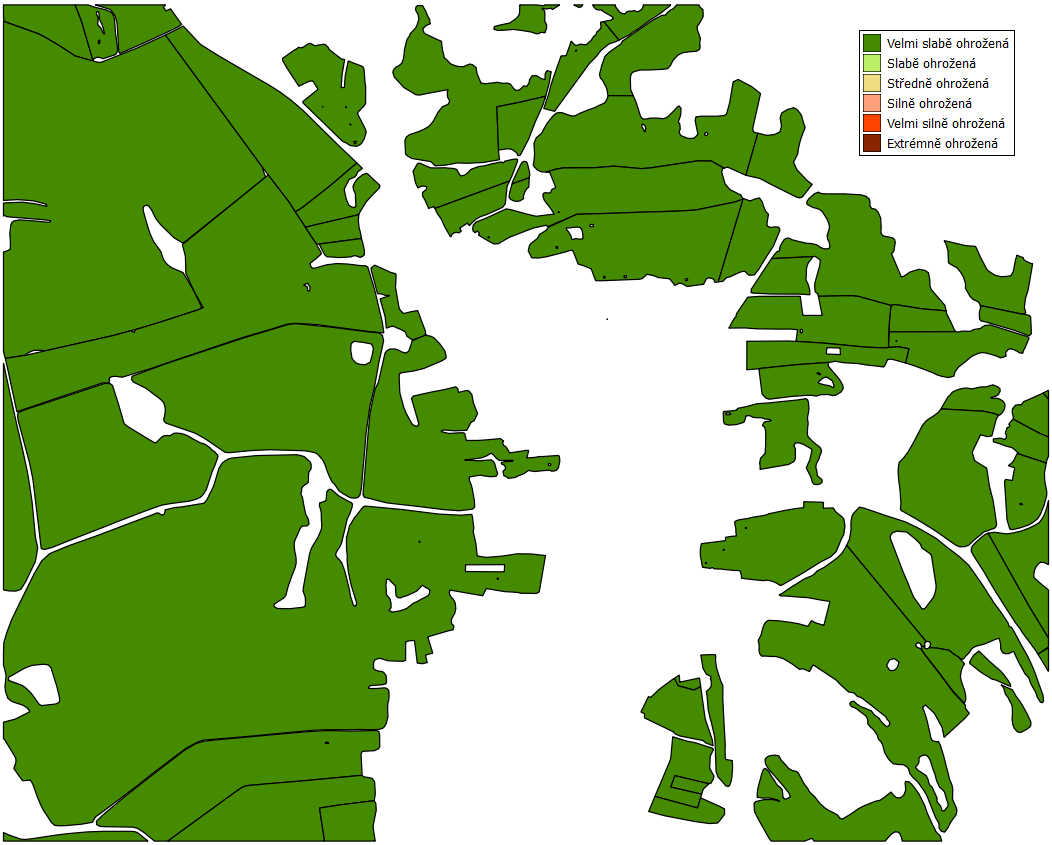
\includegraphics[width=.5\textwidth]{./pictures/euc_layer.png}
		\caption[Vrstva EUC]{Vrstva EUC, zdroj: autor}
		\label{euc_sample}
\end{figure}
\paragraph{Poznámka:} Výsledná vrstva EUC je jednolitá z důvodu nízké
erozní ohroženosti oblasti. Tato oblast ovšem musela být vybrána z
důvodu využití vzorových (volně šiřitelných) dat DMT z DMR 5G.
\begin{figure}[H] \centering
		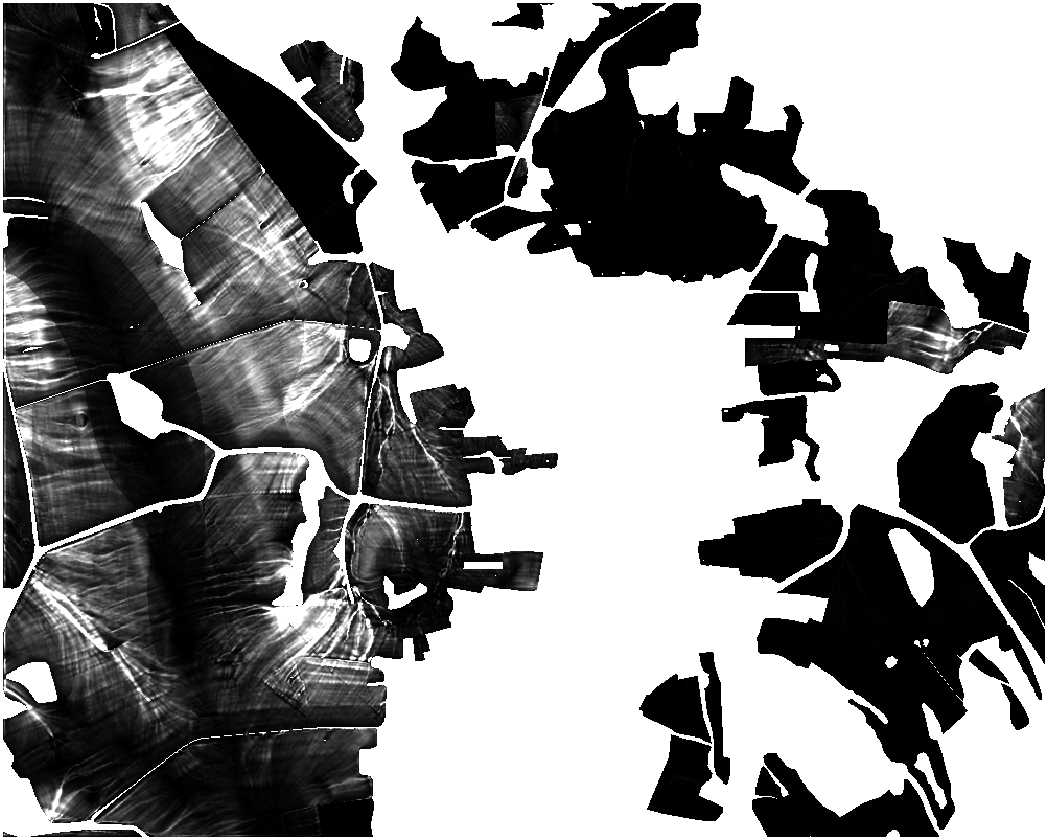
\includegraphics[width=.5\textwidth]{./pictures/lokalni_eroze_layer.png}
		\caption[Vrstva G faktor]{Vrstva G faktor, zdroj:
autor}
		\label{g_sample}
              \end{figure}
              
%%% ML: text nize bych v priloze neuvadel
              
% \section{Autoři} Pro Labolatoř GeoForAll - České vysoké učení
% technické v Praze

% Jako bakalářskou práci vytvořil Radek Novotný pod vedením Ing. Martina
% Landy, PhD.

% Konec dokumentu
\end{document}
